\documentclass[bibtotoc,liststotoc,BCOR=5mm,DIV=12]{scrbook}

% use this declaration to set specific page margins
%\usepackage[a4paper , lmargin = {2.7cm} , rmargin = {2.9cm} , tmargin = {2.7cm} , bmargin = {4.6cm} ]{geometry}
\usepackage[a4paper]{geometry}

\usepackage[ngerman, english]{babel}
\usepackage{bibgerm}       		% german references
\usepackage[T1]{fontenc} % german characters
\usepackage{graphicx} 				% it's recommended to use PDF images but you can use JPG or PNG as well
\usepackage{url}           		% format URLs
\usepackage{hyperref} 				% create hyperlinks
\usepackage{listings, color}	% for source code
\usepackage{subfig}						% two figures next to each other (example: figure 3a), figure 3b)
\usepackage{scrlayer-scrpage}					% header and footer line
\usepackage{todonotes}
% header and footer line - no header & footer line on pages where a new chapter starts
\pagestyle{scrheadings}
\ohead{Design and Implementation of X}
\ihead{Your Name}
\ofoot[]{\thepage}
\ifoot{Thesis, TU Berlin, Fachgebiet ISE, 2019}

% set path where images are stored
\graphicspath{{./img/}}

%
% der Befehl \hypenation versteht keine Sonderzeichen, also weder ä
% noch "a noch \"a. Wörter die derartige Zeichen enthalten müssen
% direkt im Text getrennt werden, z.B. Wör\-ter
%
\hyphenation{te-le-com-muni-cation 
te-le-com-muni-cation-specific 
Te-le-kom-mu-ni-ka-tions-API} 					% use this file to set explicit hyphenations (doesn't seem to work correctly)

\begin{document}
% ---------------------------------------------------------------
\frontmatter
    \thispagestyle{empty}
\begin{center}

\vspace*{1.4cm}
{\LARGE \textbf{Technische Universität Berlin}}

\vspace{0.5cm}

{\large Information Systems Engineering\\[1mm]}

Fakultät IV\\
Einsteinufer 17\\
10587 Berlin\\
https://www.tu.berlin/ise\\

\vspace*{1cm}


\includegraphics[width=4cm]{tu_logo}

\vspace*{1.0cm}

{\LARGE Master Thesis}\\

\vspace{1.0cm}
{\LARGE \textbf{Design, Implementation and Evaluation}}\\
\vspace*{0.3cm}
{\LARGE \textbf{of Zero Knowledge Rollups using the ZoKrates Toolbox}}\\
\vspace*{1.0cm}
{\LARGE De Tomasi Andrea}
\\
\vspace*{0.5cm}
Matriculation Number: 1234567\\
01.01.2010\\ % 	date of submission
\todo[inline]{Add matriculation and submission date}
\vspace*{1.0cm}

Supervised by\\
Prof. Dr. Stefan Tai\\
Prof. Dr. \todo{2nd supervisor}

\vspace*{0.5cm}
Assistant Supervisor\\
\todo[inline]{fill with assistant supervisor}
\vspace{3cm}


\end{center}


    \thispagestyle{empty}
    \cleardoublepage
    
    
    \newpage

\thispagestyle{empty}

\begin{large}

\vspace*{6cm}

\noindent
Hereby I declare that I wrote this thesis myself with the help of no more than the mentioned literature and auxiliary means.
\vspace{2cm}

\noindent
Berlin, 01.01.2050

\vspace{3cm}

\hspace*{7cm}%
\dotfill\\
\hspace*{8.5cm}%
\textit{(Signature \todo{[your name]})}

\end{large}
 
    \thispagestyle{empty}
    \cleardoublepage
    
    
    \thispagestyle{empty}
\vspace*{1.0cm}

\begin{center}
    \textbf{Abstract}
\end{center}

\vspace*{0.5cm}

\noindent
This template is intended to give an introduction of how to write diploma and master thesis at the chair 'Architektur der Vermittlungsknoten' of the Technische Universität Berlin. Please don't use the term 'Technical University' in your thesis because this is a proper name. 
\\
\\
On the one hand this PDF should give a guidance to people who will soon start to write their thesis. The overall structure is explained by examples. On the other hand this text is provided as a collection of LaTeX files that can be used as a template for a new thesis. Feel free to edit the design.
\\
\\
It is highly recommended to write your thesis with LaTeX. I prefer to use Miktex in combination with TeXnicCenter (both freeware) but you can use any other LaTeX software as well. For managing the references I use the open-source tool jabref. For diagrams and graphs I tend to use MS Visio with PDF plugin. Images look much better when saved as vector images. For logos and 'external' images use JPG or PNG. In your thesis you should try to explain as much as possible with the help of images.
\\
\\
The abstract is the most important part of your thesis. Take your time to write it as good as possible. Abstract should have no more than one page. It is normal to rewrite the abstract again and again, so  probaly you won't write the final abstract before the last week of due-date. Before submitting your thesis you should give at least the abstract, the introduction and the conclusion to a native english speaker. It is likely that almost no one will read your thesis as a whole but most people will read the abstract, the introduction and the conclusion.
\\
\\
Start with some introductionary lines, followed by some words why your topic is relevant and why your solution is needed concluding with 'what I have done'. Don't use too many buzzwords. The abstract may also be read by people who are not familiar with your topic.
    \thispagestyle{empty}
    \cleardoublepage
    
    \thispagestyle{empty}
\vspace*{0.2cm}

\begin{center}
    \textbf{Zusammenfassung}
\end{center}

\vspace*{0.2cm}

\noindent 
Da die meisten Leuten an der TU deutsch als Muttersprache haben, empfiehlt es sich, das Abstract zusätzlich auch in deutsch zu schreiben. Man kann es auch nur auf deutsch schreiben und anschließend einem Englisch-Muttersprachler zur Übersetzung geben.
    \thispagestyle{empty}
    
    
    \tableofcontents
    \thispagestyle{empty}
    
    \todo[inline]{talk to your supervisor if this is needed}
    \listoffigures
    \thispagestyle{empty}
    
    \listoftables
    \thispagestyle{empty}
    
% --------------------------------------------------------------

\mainmatter % comment single chapters for faster compilation

    \chapter{Introduction}\label{cha:chapter1}

This chapter provides an overview of the motivation, context, and objectives of the thesis.

\section{Motivation}\label{sec:moti}

In recent years, blockchain technology has witnessed remarkable growth, with the introduction of Bitcoin in 2008 \cite{nakamoto_bitcoin_2008} marking the emergence of a decentralized, distributed ledger concept. Since then, numerous blockchains with unique features have been developed, gaining widespread popularity.

As the popularity of blockchains continues to rise, many companies are exploring the technology's potential and attracting new users. Predictions indicate exponential growth in the blockchain space in the coming years \cite{noauthor_global_nodate}. However, this growth presents a challenge due to the limited scalability offered by current blockchains. For instance, Ethereum, one of the most popular blockchains, currently faces a transaction processing limit of only 15 transactions per second (TPS).

The necessity for blockchain scalability has been recognized by the community, especially evident when Ethereum transaction fees reached an average of \$70 in 2020\footnote{\url{https://ycharts.com/indicators/ethereum_average_transaction_fee}} due to the high volume of submitted transactions and consequent congestion of the network. This issue is not unique to Ethereum, as other blockchains also experience similar problems. Vitalik Buterin's "Scalability Trilemma" posits that achieving scalability, security, and decentralization simultaneously in a distributed system, such as blockchains, is a challenging task\footnote{\url{https://ethereum.org/en/roadmap/vision/}}.

\section{Objective}\label{sec:objective}

The objective of this thesis is to address the issue of limited scalability and high fees in the blockchains. A crucial factor that constrains the number of transactions in a block is the gas limit. The gas limit serves as a hard limit on the computational work that can be performed within a block, measured in gas units. Each transaction and contract interaction, in fact, consumes gas, and the gas limit determines the maximum amount of computational availability.

The gas limit mechanism is essential for preventing infinite loops in a smart contract execution and defending against denial-of-service attacks. It's also necessary to ensure that a minimal number of transactions can be included in the block. However, it can also hinder the proper execution of a program that intentionally involves extended computations \cite{wood_ethereum_nodate}.

Enhancing the blockchain's throughput is also directly impacted by the block size, as increasing its size can increase the system's capacity. Nonetheless, a thorough analysis of the consequences of enlarging the block size is necessary, as arbitrary increases can lead to negative effects. For instance, large block sizes may cause network congestion, slower propagation speeds, and an increase in the number of stale blocks—blocks that are not included in the longest chain due to conflicts or concurrency—posing potential security risks \cite{gervais_security_2016}.

This thesis proposes a solution to the scalability problem by introducing a new block-chain Layer that lives on top of the original blockchain. This is called a Layer 2 solution (L2). This second Layer is entirely run by nodes that are not involved in computing or verifying Layer 1 transactions. This way we are not constrained by limitations imposed by the chain, like the gas limit or block size, but we are free to use a lot more computational power. Rollups, a Layer 2 solution, in fact inject into the blockchain only the result of the computations performed outside the chain, making use of the unconstrained computational availability offered on L2. With this approach it should be possible to achieve higher throughput when congestion occurs and lower transaction fees. 

\section{Research Questions}

\section{Structure\label{sec:structure}}

\todo[inline]{Change}

This section gives a brief introduction into the main chapters of this thesis. 
\\
\\
\textbf{Chapter \ref{cha:chapter2}} analyzes the current state of the art in the field of blockchain scalability and presents the most relevant related work including the project this thesis is based on.
\\
\\
\textbf{Chapter \ref{cha:chapter3}} analyzes the research question and the requirements for the Rollup System.
\\
\\
\textbf{Chapter \ref{cha:chapter4}} describes the architecture of the Layer 1 and Layer 2 components. It also describes the communication between the two layers.
\\
\\
\textbf{Chapter \ref{cha:chapter5}} describes the implementation part of the Rollup System.It shows the components and the technologies used to build the system. It also describes the challenges faced during the development.
\\
\\
\textbf{Chapter \ref{cha:chapter6}} shows the tests performed and the results obtained. It also shows the limitations of the system and the possible future improvements.
\\
\\
\textbf{Chapter \ref{cha:chapter7}} summarizes the work done and the challenges faced. It presents the conclusions and the future work to improve the system.

    \chapter{State of the Art \& Related Work}
\label{cha:chapter2}

This chapter provides an overview of the prominent solutions in the realm of blockchain scalability and introduces the foundational project upon which this thesis is built.

\section{Scalability Approaches}
Various strategies are being explored to enhance blockchain scalability. Some are already operational, while others are in the research stage. These strategies broadly fall into two categories: Layer 1 and Layer 2 solutions \cite{tyagi_study_2021,thibault_blockchain_2022}. Layer 1 solutions focus on boosting blockchain scalability through means like enlarging block sizes or implementing Sharding. In contrast, Layer 2 solutions endeavor to scale the blockchain by relocating computation off-chain. Noteworthy examples of Layer 2 solutions encompass State Channels, Sidechains, and Rollups, as illustrated in Figure \ref{fig:2_scalingSolutions}.

The prevailing trajectory for blockchain scalability involves the adoption of Layer 2 solutions. This course of action is being embraced by a significant portion of the Ethereum community \cite{neiheiser_practical_2023}.

\begin{figure}[ht]
  \centering
  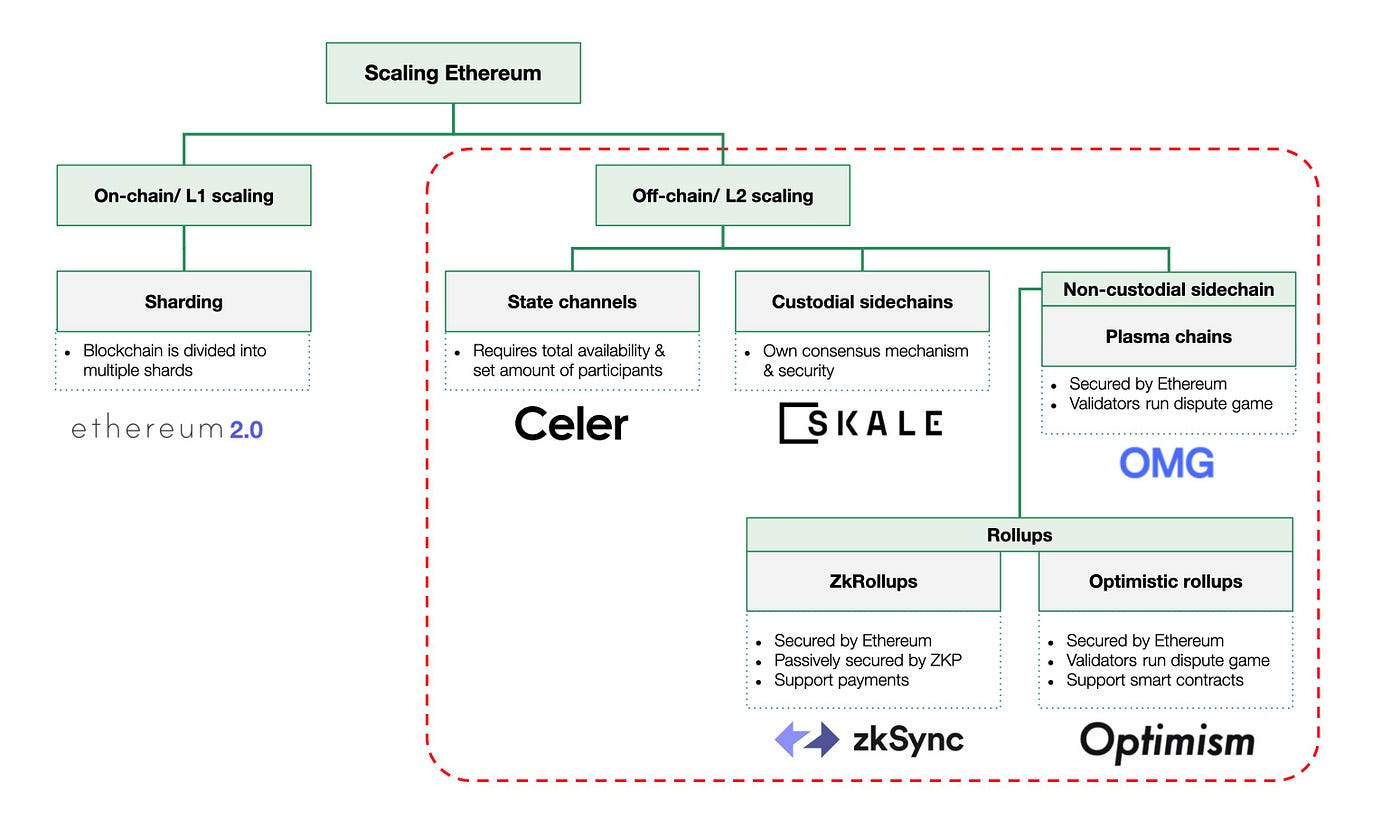
\includegraphics[width=0.95\columnwidth]{2_scalingSolutions.jpg}
  \caption[Scaling Solutions]{Principal scaling solutions for Layer 1 and Layer 2\footnotemark}  
  \label{fig:2_scalingSolutions}
\end{figure} 
\footnotetext{\url{https://medium.com/token-terminal/a-primer-on-ethereum-l2-scaling-techniques-17ac437891b1}}

\subsection{Zk-Rollups}
\label{sec:2_zkRollups}
Zk-Rollups represent a Layer 2 approach that leverages zero-knowledge proofs to conduct computation off-chain. Post-computation outcomes and a proof of verifiably correct execution are transmitted to the blockchain's smart contract. The smart contract then verifies the proof before incorporating the results onto the blockchain \cite{tyagi_study_2021}.

Figure \ref{fig:2_zkRollup_schema} outlines the Zk-Rollup paradigm. An user initiates a transaction with the off-chain node. The node processes the transaction batch, using the state fetched from the blockchain, and relays results and proof to the smart contract. Following proof validation, the new account balance list is recorded on the blockchain.

\begin{figure}[ht]
  \centering
  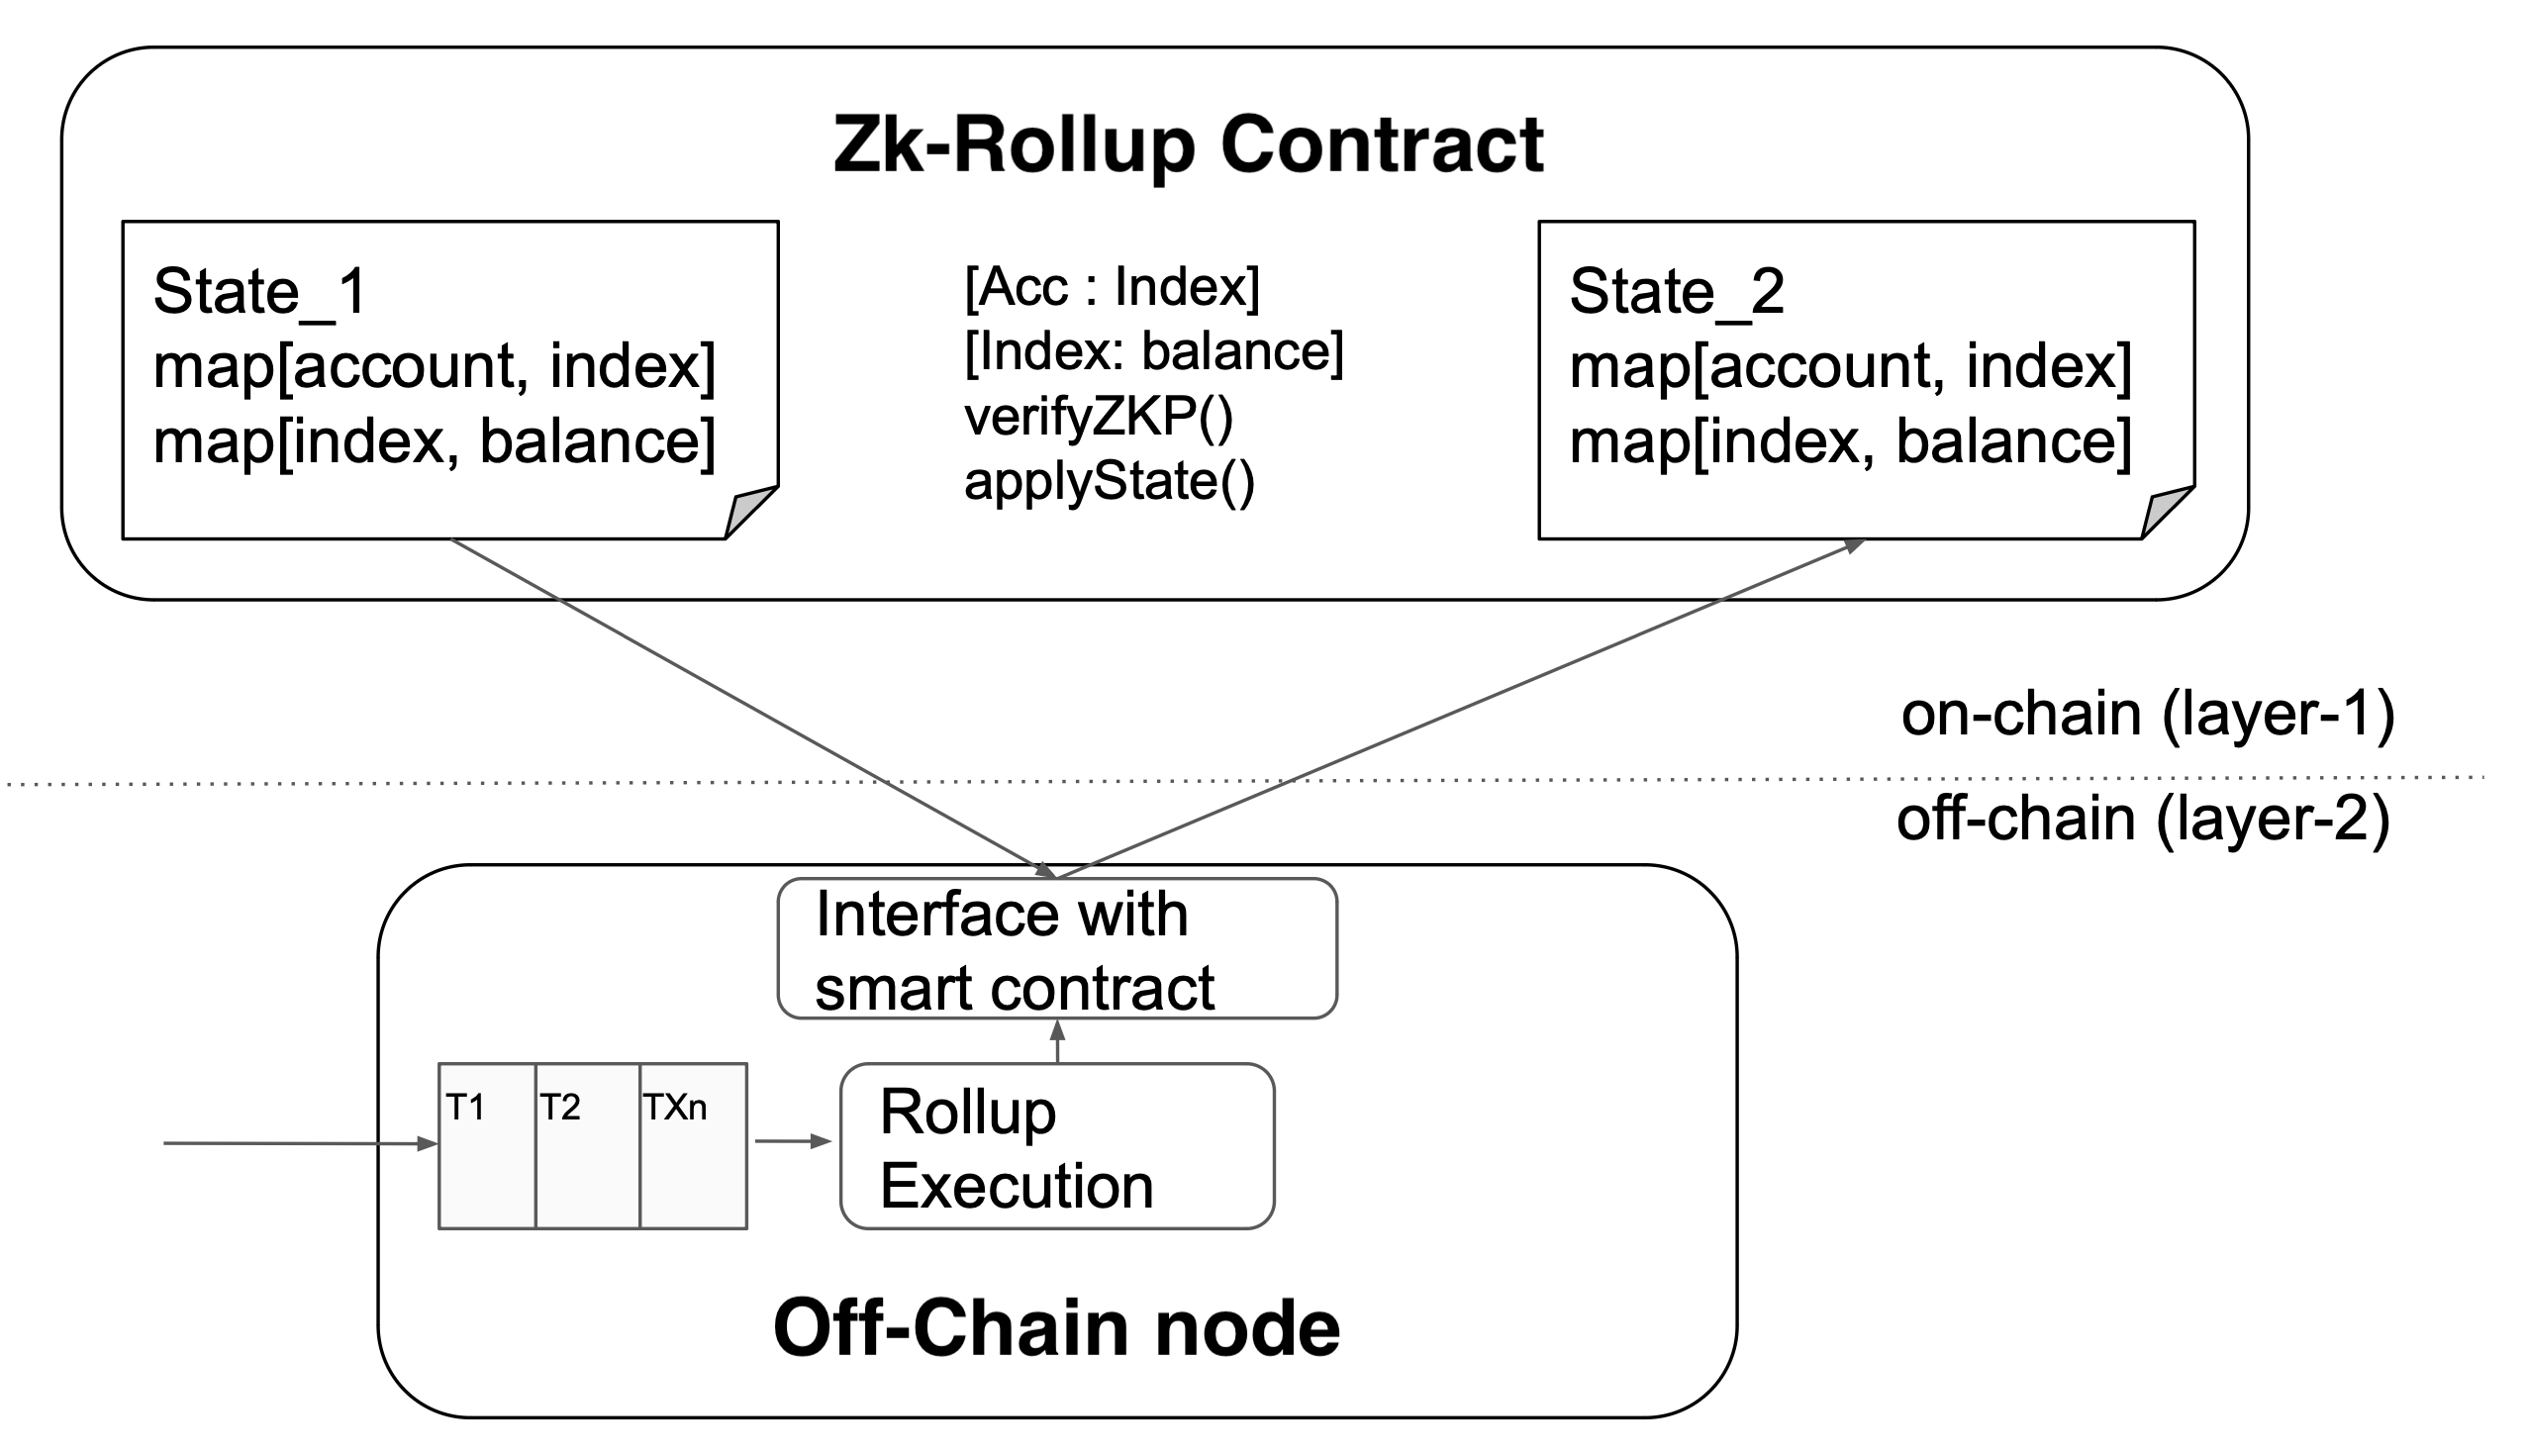
\includegraphics[width=0.95\columnwidth]{2_zkRollup_architecture.png}
  \caption[Zk-Rollup Schema]{General schema of a Zk-Rollup\cite{ise_department_tub_material_nodate}}  
  \label{fig:2_zkRollup_schema}
\end{figure}

\subsection{ZoKrates}
ZoKrates is a toolbox for zkSNARKs on Ethereum: it allows developers to write zero-knowledge proofs in a high-level programming language and generate trusted setup parameters and zero-knowledge proofs \cite{eberhardt_ZoKrates_2018}.

\todo[inline]{explain ZoKrates}

\section{ADSP Project: Scaling Tezos Blockchain with Zk-Rollups}
In the Winter Semester 2022/2023 at the University of Berlin, I collaborated with the ADSP (Advanced Distributed Systems Prototype) group on a project. The project's objective was to scale the Tezos blockchain using Zk-Rollups through the ZoKrates toolbox.

The group partially achieved the project's objectives, creating a proof of concept. The system architecture features Layer 1 and Layer 2 components: Layer 1 includes two smart contracts for state management and proof verification; Layer 2 encompasses a node executing transactions within the ZoKrates program, generating proofs for the smart contract. Figure \ref{fig:2_general_rollup_architecture} offers an overview of the entire system.

\begin{figure}[ht]
  \centering
  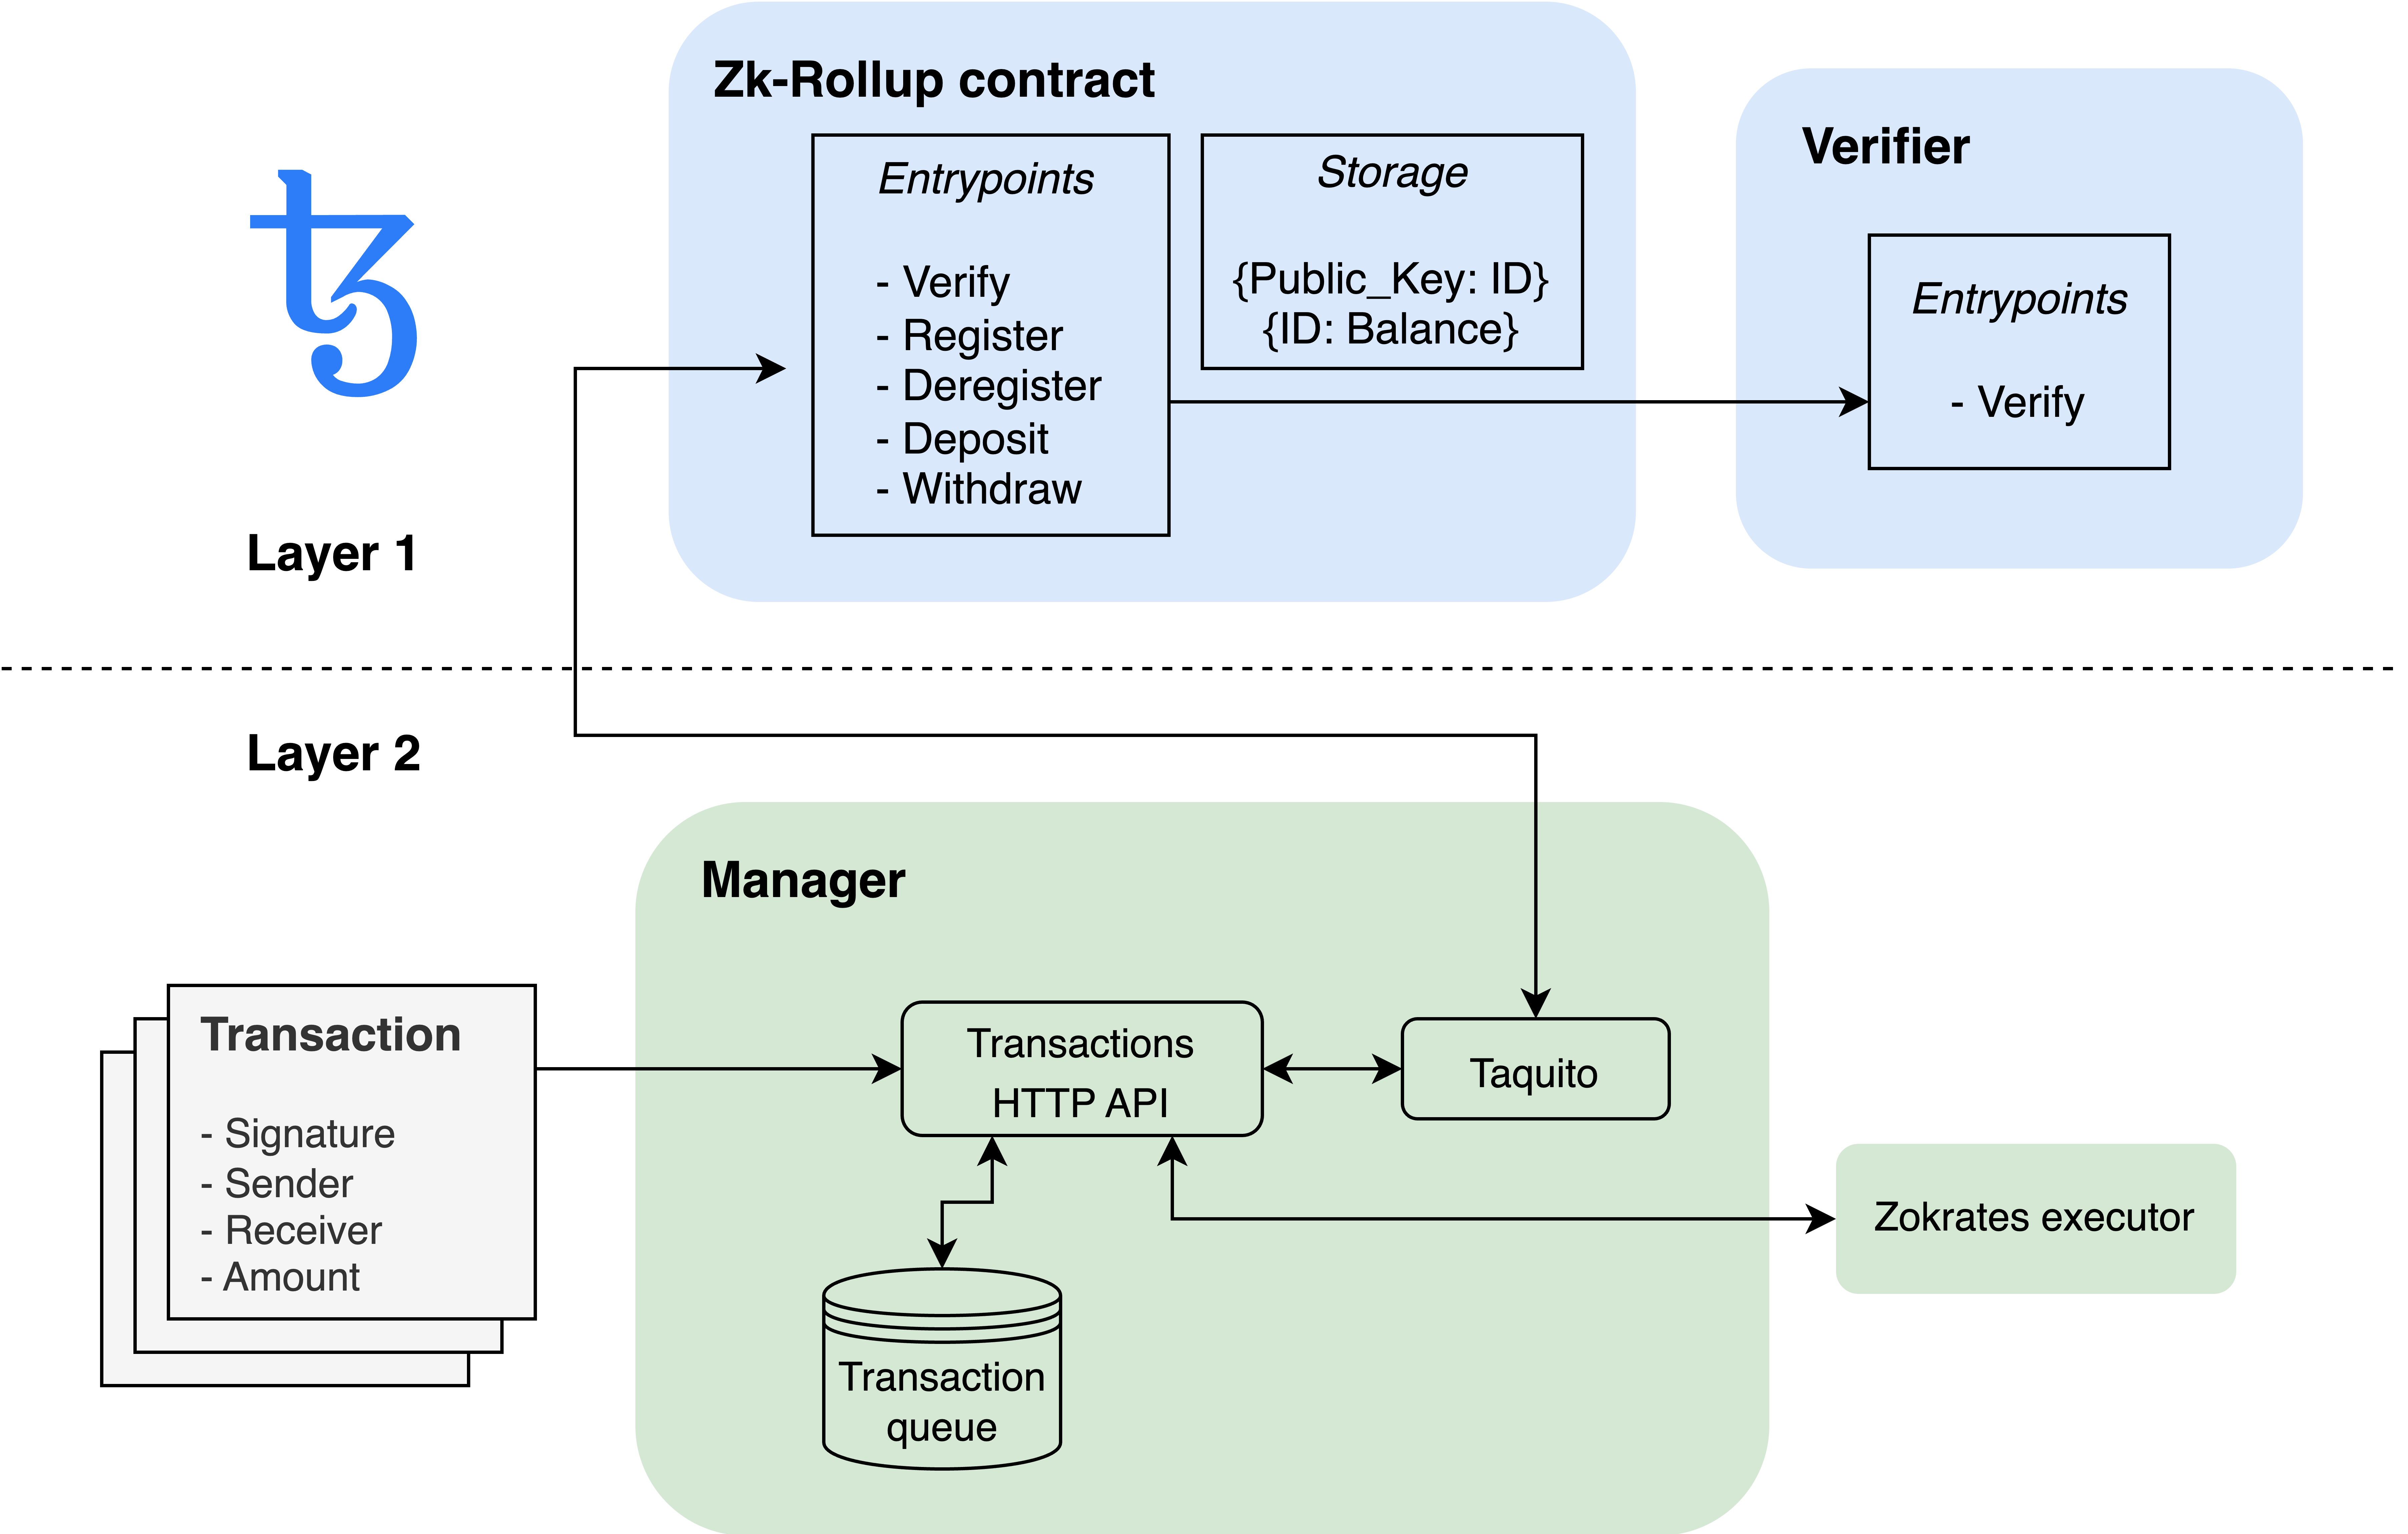
\includegraphics[width=0.95\columnwidth]{2_drawings-adsp_rollup_architecture.png}
  \caption[Zk-Rollup Architecture]{General Zk-Rollup architecture}  
  \label{fig:2_general_rollup_architecture}
\end{figure}

The Zk-Rollup execution process unfolds as follows:
\begin{enumerate}
    \item A user dispatches a transaction to the off-chain node, managed by a NodeJS server (the manager);
    \item The manager logs the transaction in a transaction queue;
    \item Once three transactions accumulate, the node processes the transaction batch, spawning the ZoKrates executor;
    \item The manager fetches the current state from the Tezos Zk-Rollup smart contract;
    \item The ZoKrates executor processes the ZoKrates program with the transaction batch and the current state as input;
    \item The ZoKrates executor generates a proof and new balance list, transmitting them to the NodeJS server;
    \item The NodeJS server converts ZoKrates outputs into a Tezos-compatible format;
    \item Converted outputs are dispatched to the Tezos Zk-Rollup smart contract;
    \item The smart contract forwards the proof to the verifier smart contract;
    \item The verifier smart contract verifies the proof, communicating the result to the contract;
    \item If the proof is verified, the new balance list is stored in the Zk-Rollup contract's blockchain storage.
\end{enumerate}

Figure \ref{fig:2_drawings-adsp_sequence_general.png} illustrates the sequence of events in the Zk-Rollup execution process.

\begin{figure}[ht]
  \centering
  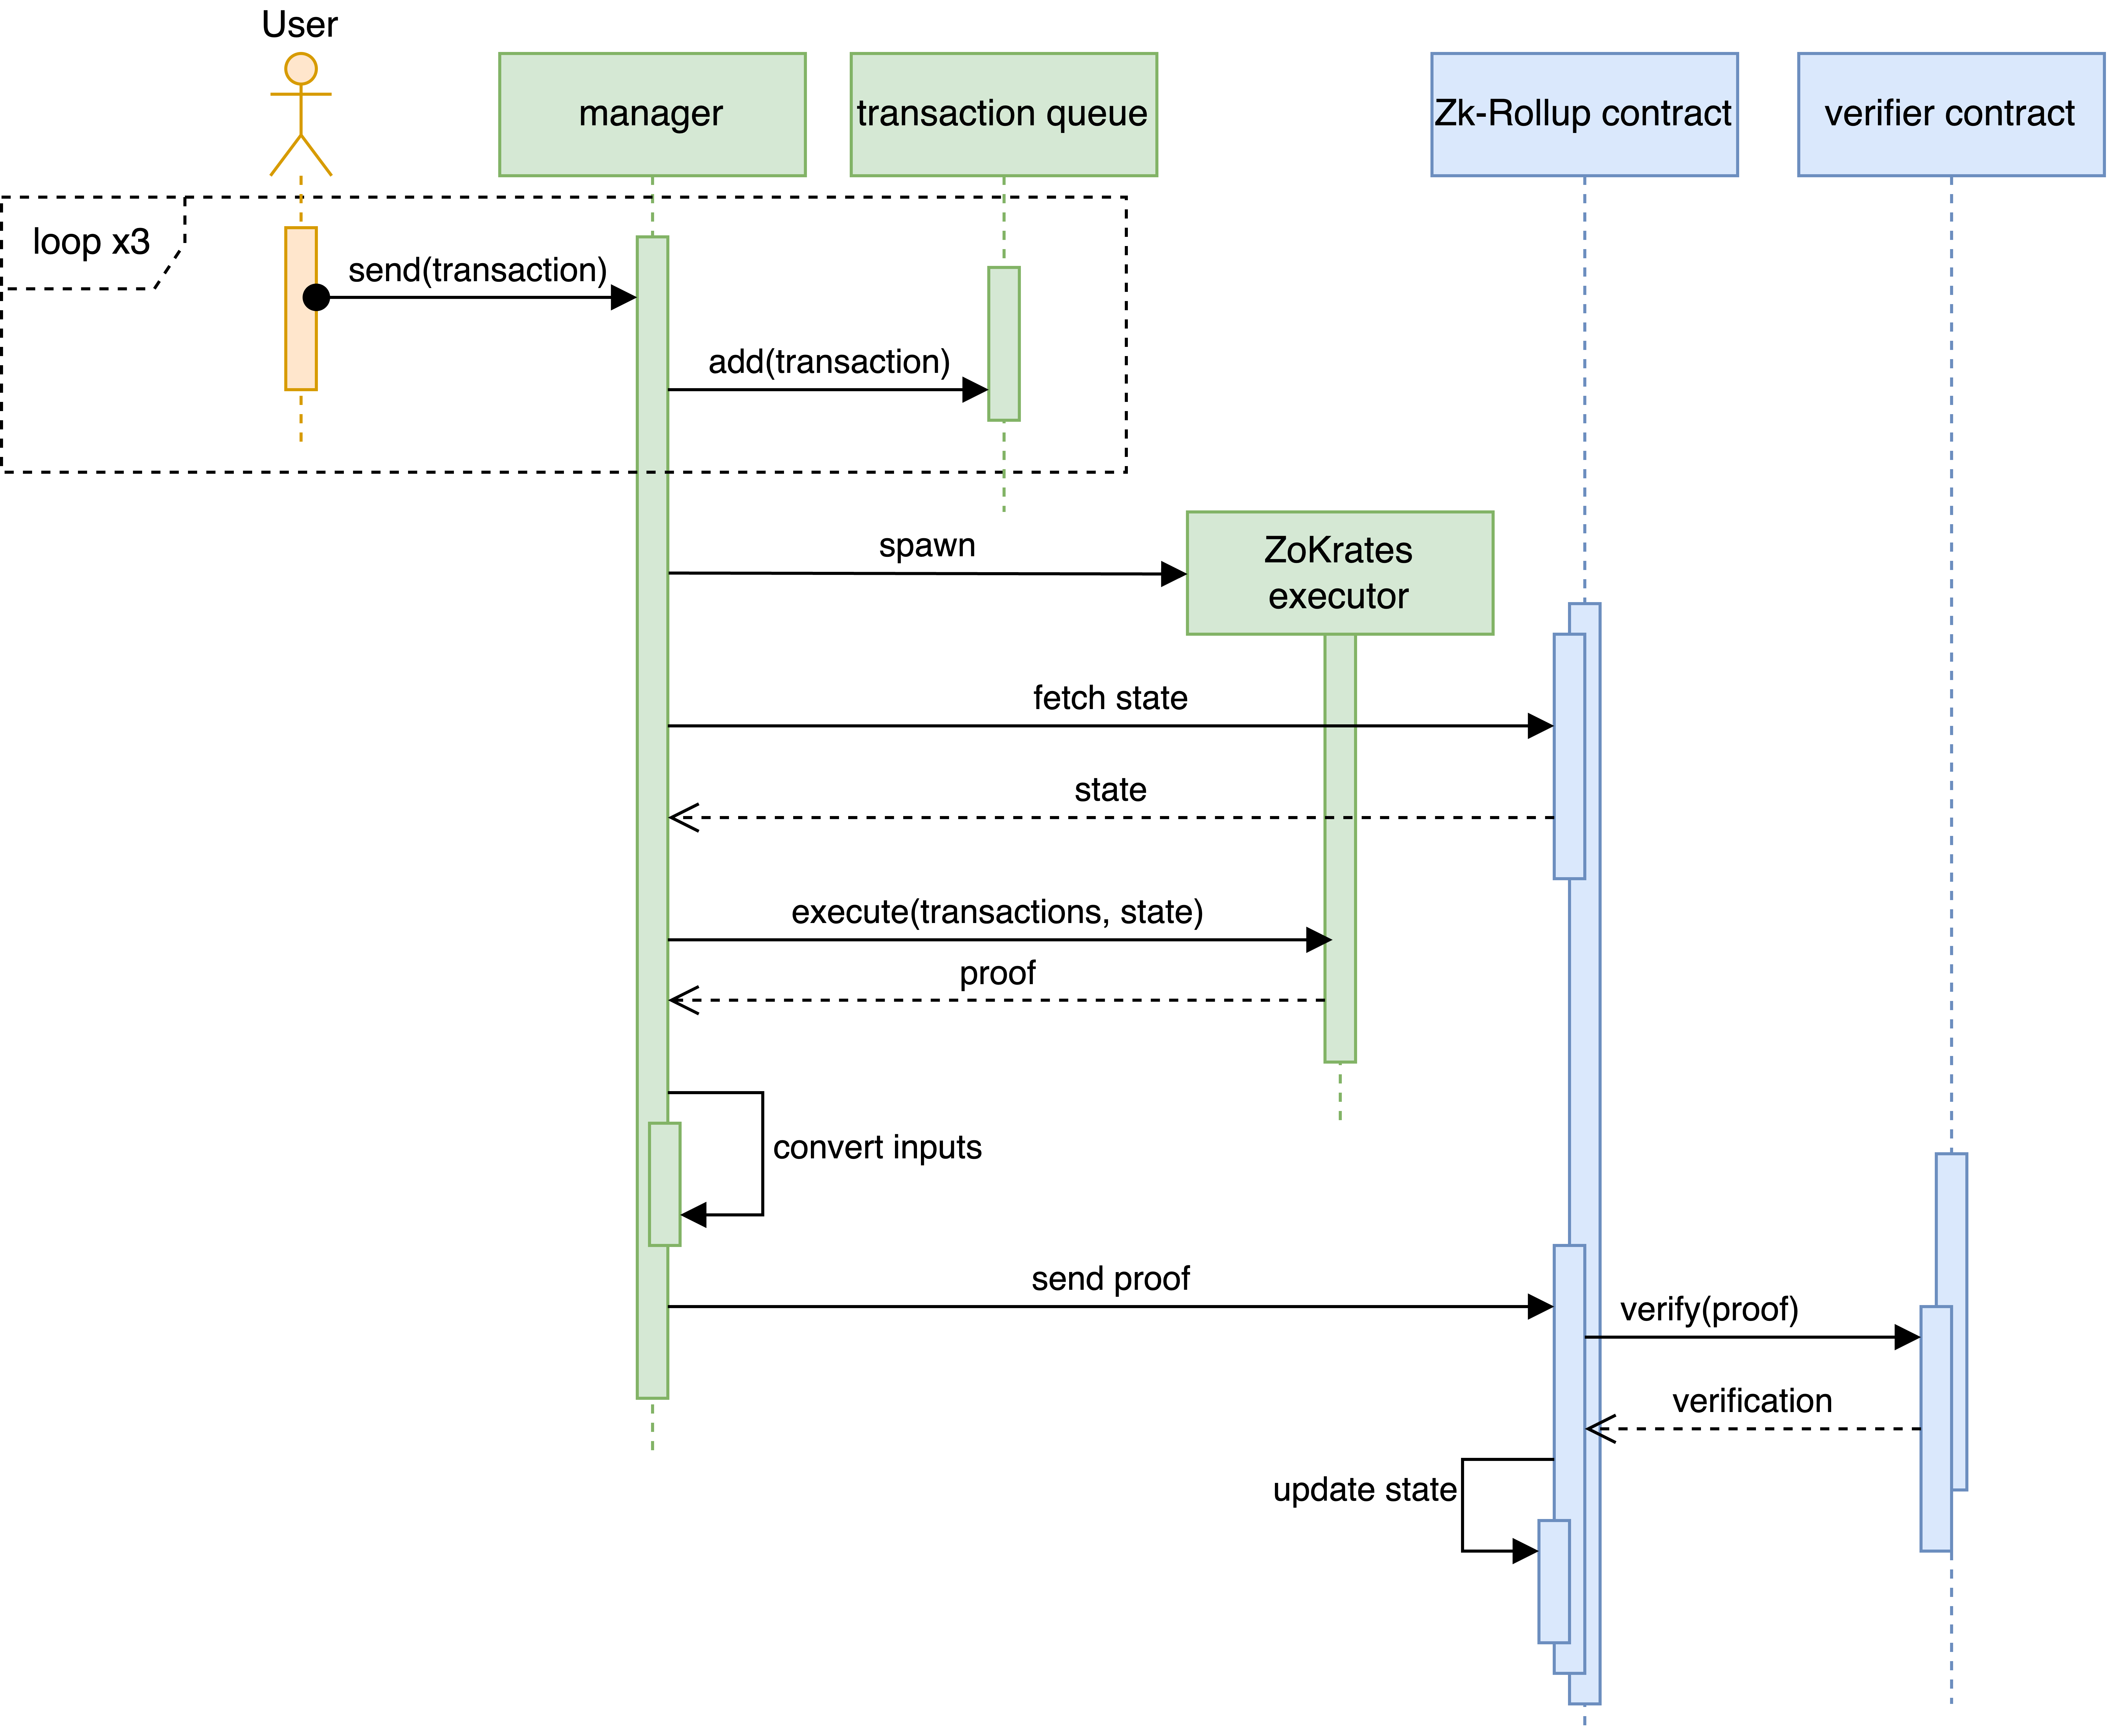
\includegraphics[width=1\columnwidth]{2_drawings-adsp_sequence_general.png}
  \caption[Scaling Solutions]{Sequence diagram of the Zk-Rollup execution process.}  
  \label{fig:2_drawings-adsp_sequence_general.png}
\end{figure} 

\subsection{Developed Components}
The team successfully implemented the Zk-Rollup \textit{Verify} entrypoint within the \textit{Zk-Rollup contract}, along with the \textit{NodeJS Manager}. Additionally, the storage mechanism was correctly executed.

The ZoKrates program was partially developed, including:
\begin{itemize}
    \item Verification of account inclusion in the rollup system;
    \item Verification of sufficient balance in sender account;
    \item Transaction execution;
    \item Generation of new balance merkle tree root, balance list, and proof.
\end{itemize}

The generation of the Merkle tree root is accomplished through the algorithm described below. This process utilizes the SHA2-256 hash function with automatic zero-padding. The algorithm incorporates pre-calculated values for the Merkle tree depth and the number of leaf nodes.

\textbf{Algorithm 1: Merkle Tree Root Generation}
\begin{lstlisting}[language=Python]
for i in 0...TREE_DEPTH {
  step_size = 2 ** (i + 1)
  step_number = LEAFS_NUM / step_size
  for j in 0...step_number {
    leftIndex = j * step_size
    rightIndex = leftIndex + step_size / 2
    leafs[leftIndex] = hash(
        leafs[leftIndex],
        leafs[rightIndex]
    )
  }
}
return leafs[0]
\end{lstlisting}

\subsection{Pending Components\label{subsec:pendingcomponents}}
Numerous aspects of the project remain unfinished, including:
\begin{itemize}
  \item Registration entrypoint;
  \item Deregistration entrypoint;
  \item Deposit entrypoint;
  \item Withdrawal entrypoint;
  \item Integration of signature checks within the ZoKrates program;
  \item Addressing the double spending issue;
  \item System optimization.
\end{itemize}
Furthermore, the project lacks a benchmarking study, a security analysis, and a cost comparison with alternative scaling solutions and Layer 1.

\todo[inline]{Provide a more comprehensive analysis of the project's state of the art.}

\section{Other Zk-Rollup Implementations}
Numerous Zk-Rollup implementations exist, particularly for Ethereum. The implementation discussed in \cite{dinh_implementation_2023} shares similarities with the ADSP project's approach. However, it lacks considerations for system scaling and handling multiple token types. Another example is Polygon Zero\footnote{\url{https://polygon.technology/blog/introducing-plonky2}}, which facilitates parallel execution of transactions on L2. This system blends STARK and SNARK, differing from the approach outlined in this thesis.

\section{Zk-Rollup Reviews}
Several studies have assessed the viability and performance of the Zk-Rollup system. \cite{capko_state_2022} offers an overview of prevalent zero-knowledge proofs. The ZoKrates Toolbox, utilized by the ADSP project, employs SNARK, which requires a trusted setup phase—a potential drawback compared to Transparent zk-SNARK \cite{zhou_overview_2022}. \cite{neiheiser_practical_2023} highlights the scalability bottleneck L2 solutions face due to slow L1, constraining them below theoretical L2 throughput. \cite{starkware_fractal_2021} proposes L3 to circumvent this issue.

\section{Alternative L2 Solutions}
Several Layer 2 strategies exist to scale blockchains. A brief overview follows.

Plasma: Plasma facilitates off-chain transaction processing through child chains or sidechains, connected to the main blockchain for security. Plasma chains expedite transactions but necessitate dispute resolution for potentially fraudulent actions \cite{thibault_blockchain_2022}. OMG Network\footnote{\url{https://docs.omg.network}} exemplifies a network employing Plasma.

State Channels: Off-chain payment channels, like state channels, enable direct user transactions without main blockchain interaction. They suit use cases like micropayments and gaming, affording fast, economical transactions \cite{negka_blockchain_2021}. Perun\footnote{\url{https://perun.network/wp-content/uploads/Perun2.0.pdf}} serves as an instance of state channel implementation.

Optimistic Rollups: This type assumes transaction validity, necessitating verification only during disputes. It combines swifter transactions with main blockchain arbitration \cite{thibault_blockchain_2022}.

    \chapter{Research Question \& Requirements\label{cha:chapter3}}
The goal of this Master Thesis is to complete the implementation of the Zk-Rollup project, test it under different conditions, evaluate its performances and finally show a proof of concept of the system applied to a real world application. This will bring a good understanding of the rollup system and show how it can be used and applied to other minor blockchain without many adaptations. This differs to other scaling solutions, like the ones described in \cite{yang_review_2020}, because they are developed closely to the blockchain they are applied to, limiting the future possibility to extend that solution.

\section{Completing the \textit{Scale Tezos Blockchain with Zk-Rollups} project}
The first goal of this Master Thesis is to finish the implementation of the Zk-Rollup project started during the Winter Semester 2022/2023 at the University of Berlin. This includes the implementation of all the missing points of the project listed at \ref{subsec:missingParts}. The partially already answered research question for this project is: \textit{How can an efficient Zk-Rollup system be implemented for the Tezos Blockchain?}

The rollup system must be capable of being usable for many applications, so it has to be developed keeping in mind to have it the most extensible, modular and blockchain agnostic as possible. This is a key concept that makes it possible to extend it in the future, implementing new features and optimizations.

\section{Scaling the Zk-Rollup system}
The second research area of this Master Thesis must answer the question: \textit{How can the previously implemented  Zk-Rollup system scale when facing a fluctuating number of users?}

It is in fact important to understand how can the system scale: horizontally, adding more nodes to increase the throughput and decentralization of the system; vertically assigning more compute capabilities to the machines; applying algorithms to distribute the load between the nodes.

This research question is a key concept to make the system usable in a real world application, when the number of users is not constant, but it can vary a lot in a short period of time while the system must be able to handle it.

\section{Proof of concept of the Zk-Rollup system applied to a NFT Marketplace}
The last area to explore is guided by the question: \textit{How can the Zk-Rollup system be applied to a real world application?}

The application chosen for this proof of concept is a NFT Marketplace. It has been chosen because the transfers involve tokens and the ownerships of the NFTs through an IPFS system. The NFTs must be handled by the application without sacrificing the decentralization of the system. This type of marketplace has also a fluctuating number of users and transactions, involving the same NTFT object, so it is a valid example to test the system applied on a real world application.

\section{Smart Contracts Requirements}

The smart contracts and layer 2 programs should prioritize system extensibility and modularity. They must be designed to efficiently handle a large number of users and transactions. However, when developing using smart contracts and zk proofs, certain constraints must be taken into account.

\subsection{Computation Gas Limit}

The computations executed within a smart contract are subject to a gas limit, a value set by the blockchain. The gas limit restricts the amount of computation a smart contract can perform in a transaction, preventing infinite loops and limiting computation within a single transaction. While users can set the gas limit when sending a transaction, it cannot exceed the maximum gas limit set by the blockchain. If the gas limit is reached during transaction execution, the transaction is reverted, and the user loses the gas used for computation. Currently, the Tezos blockchain sets a gas limit of 1040000 gas units for transactions\footnote{\url{https://mainnet.api.tez.ie/chains/main/blocks/4001570/context/constants}}.

\subsection{Storage Read Limit}

The rollup smart contract is responsible for storing registered accounts, balances, and associated tokens within the rollup system. While there is no specific predefined limit on the storage size, it becomes a critical factor during entrypoint execution. Upon each entrypoint call, the contract and its storage are deserialized for use by the Michelson interpreter. To avoid excessive time consumption and reaching the gas limit, it's crucial to keep the contract's storage as compact as possible. If the storage becomes too large, the contract may become unusable due to the gas limit being reached before the contract can be deserialized. A recommended solution offered by Tezos is to utilize big maps for storing data. Big maps are special maps that are only deserialized when accessed, and only the required data is loaded, allowing for more efficient storage management. However, it's important to note that iterating over big maps or determining their size is not directly supported.

    \chapter{Context \& Requirements\label{cha:chapter4}}
The goal of this Master Thesis is to complete the implementation of the Zk-Rollup project, test it under different conditions, evaluate its performances and finally show a proof of concept of the system applied to a real world application. This will bring a good understanding of the rollup system and show how it can be used and applied to other minor blockchains without many adaptations. This differs from other scaling solutions, like the ones described in \cite{yang_review_2020}: they are in fact developed closely to the blockchain they are applied to, limiting the future possibility to extend that solution.

\section{ADSP Project: Scaling Tezos Blockchain with Zk-Rollups \label{sec:2_adspProject}}

During the Winter Semester 2022/2023 at the University of Berlin, I collaborated with the Advanced Distributed Systems Prototype (ADSP) group on a project. The project's objective was to scale Tezos blockchain using Zk-Rollups through the ZoKrates toolbox.

The group partially achieved the project's objectives, creating a proof of concept. The system architecture features Layer 1 and Layer 2 components: Layer 1 includes two smart contracts for state management and proof verification; Layer 2 encompasses a node executing transactions within the ZoKrates program, generating proofs verified by the smart contract. Figure \ref{fig:3_general_rollup_architecture} offers an overview of the entire system.

\begin{figure}[ht]
  \centering
  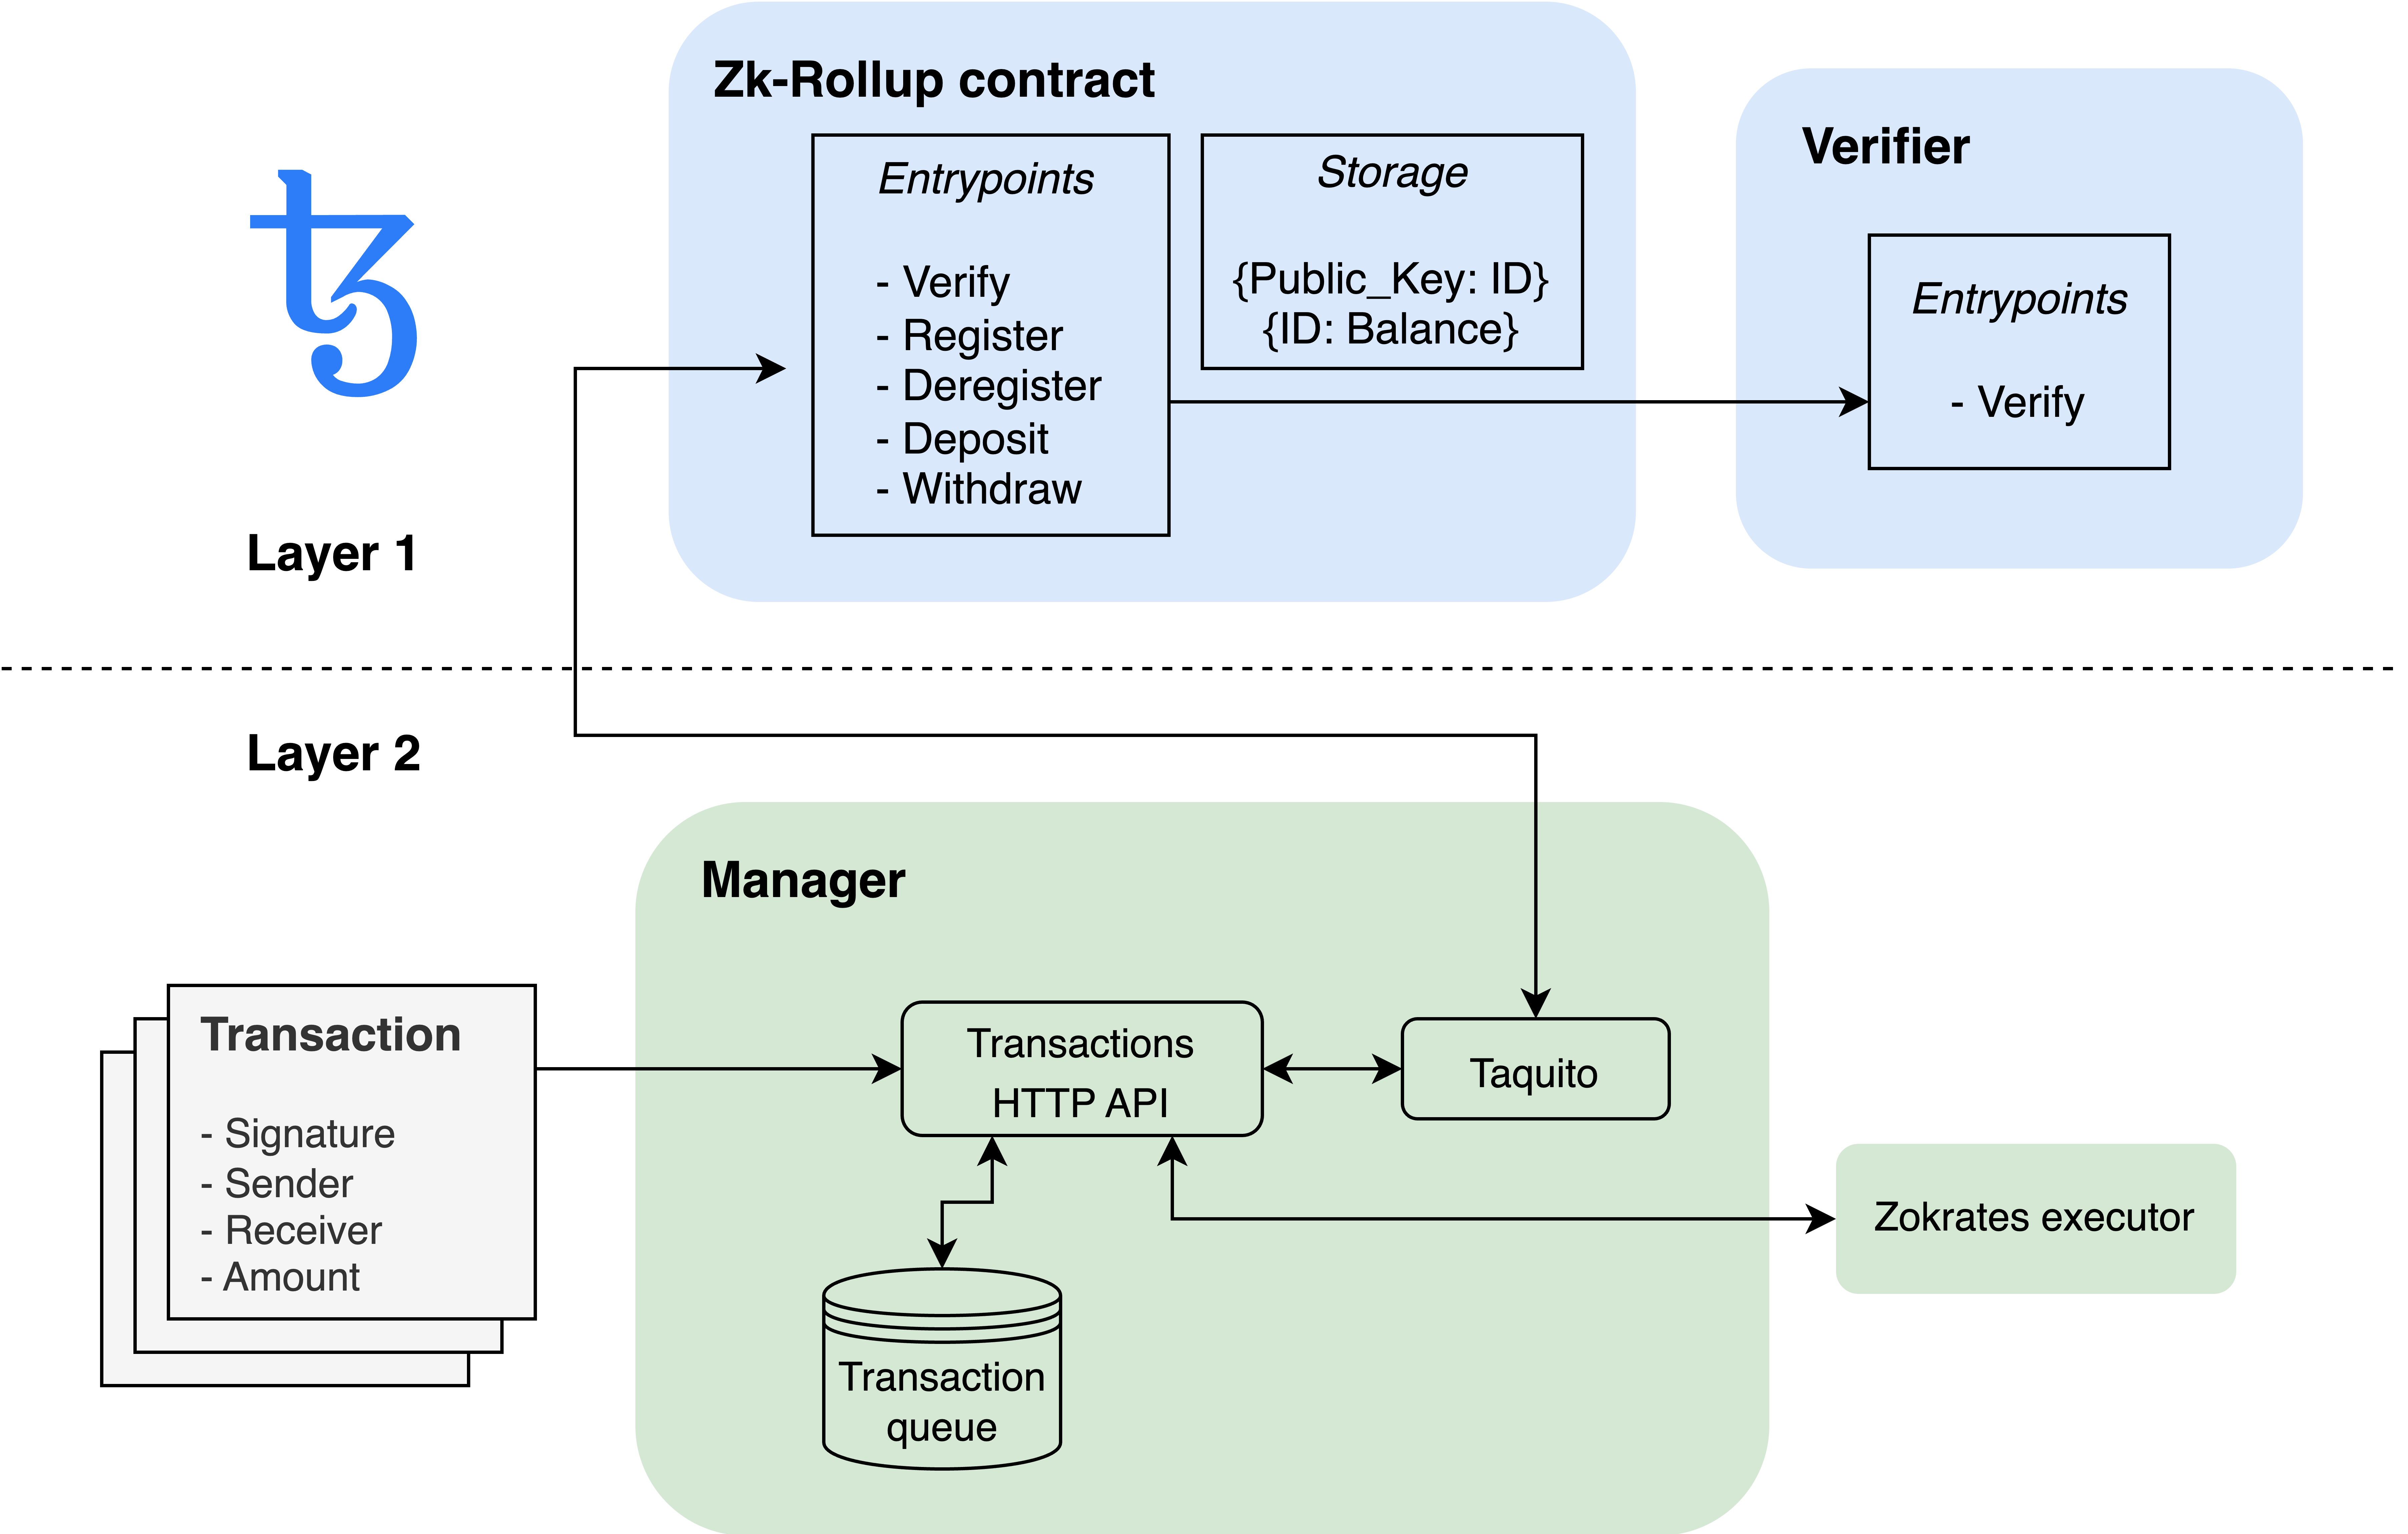
\includegraphics[width=0.95\columnwidth]{2_drawings-adsp_rollup_architecture.png}
  \caption[Project Architecture]{Project architecture}  
  \label{fig:3_general_rollup_architecture}
\end{figure}

The Zk-Rollup execution process occurs as follows:
\begin{enumerate}
    \item A user dispatches a transaction to the off-chain node, managed by a NodeJs server (the Web-Manager);
    \item The Web-Manager stores the transaction in a transaction queue;
    \item Once three transactions accumulate, the Web-Manager fetches the current state from the Tezos Zk-Rollup smart contract;
    \item The L2 node processes the transaction batch, executing the ZoKrates program using the transaction batch and the current state as input;
    \item The ZoKrates program generates a proof and new balance list;
    \item The node converts ZoKrates outputs into a Tezos-compatible format;
    \item Converted outputs are dispatched to the Tezos Rollup smart contract using Taquito, an external Typescript library;
    \item The smart contract forwards the proof to the verifier smart contract;
    \item The verifier smart contract verifies the proof, communicating the result to the Rollup-Manager contract;
    \item If the proof is verified, the new balance list is stored in the Manager contract's blockchain storage.
\end{enumerate}

Figure \ref{fig:3_drawings-adsp_sequence_general.png} illustrates the sequence of events in the Zk-Rollup execution process.

\begin{figure}[ht]
  \centering
  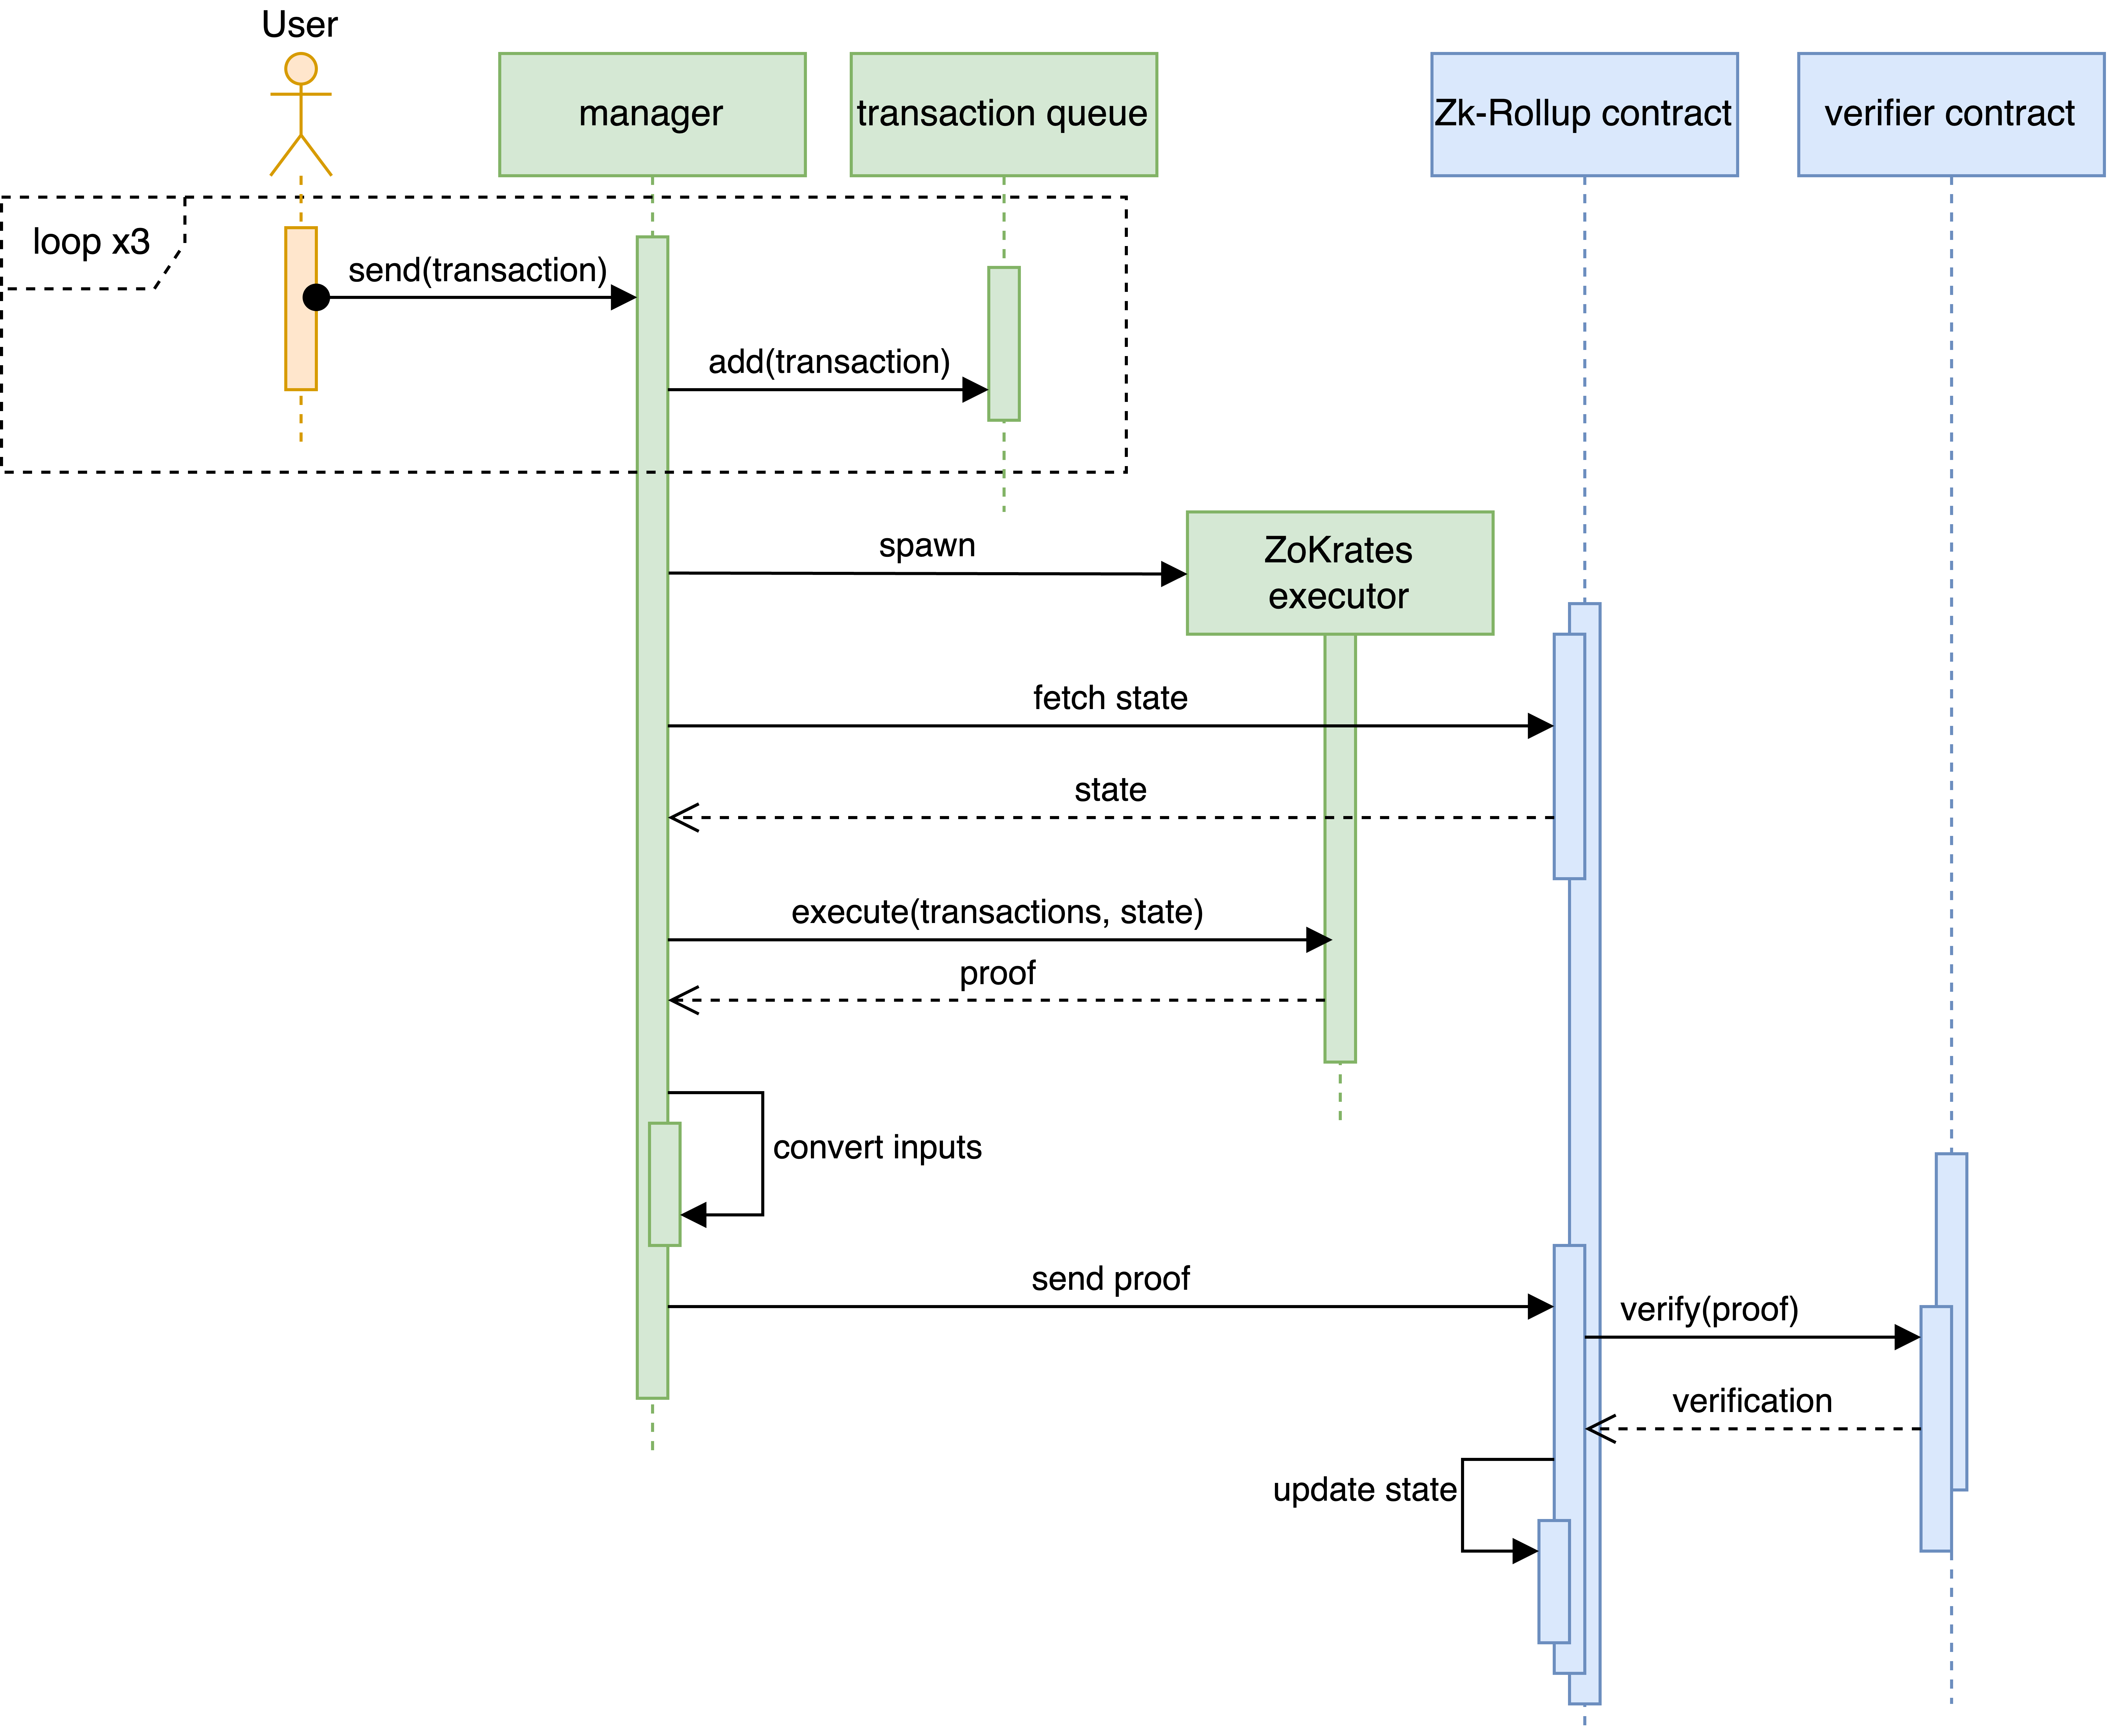
\includegraphics[width=1\columnwidth]{2_drawings-adsp_sequence_general.png}
  \caption[Sequence Zk-Rollup]{Sequence diagram of the Zk-Rollup execution process.}  
  \label{fig:3_drawings-adsp_sequence_general.png}
\end{figure} 

\subsection{Developed Components}
The team successfully implemented the Rollup-Manager \textit{Verify} entrypoint within the \textit{Rollup contract}, along with the \textit{NodeJs Manager}. Additionally, the storage mechanism was correctly executed.

The ZoKrates program was partially developed, including:
\begin{itemize}
    \item Verification of account inclusion in the rollup system;
    \item Verification of sufficient balance in sender account;
    \item Transaction execution;
    \item Generation of new balance merkle tree root, balance list, and proof.
\end{itemize}

The generation of the Merkle tree root is accomplished through the algorithm described below. This process utilizes the sha256 hash function with automatic zero-padding. The algorithm uses constant and known values for Merkle tree depth and number of leaf nodes.

\noindent\textbf{Algorithm 1: Merkle Tree Root Generation}
\begin{lstlisting}[language=Python]
for i in 0...TREE_DEPTH {
  step_size = 2 ** (i + 1)
  step_number = LEAFS_NUM / step_size
  for j in 0...step_number {
    leftIndex = j * step_size
    rightIndex = leftIndex + step_size / 2
    leafs[leftIndex] = hash(
        leafs[leftIndex],
        leafs[rightIndex]
    )
  }
}
return leafs[0]
\end{lstlisting}

\subsection{Pending Components\label{subsec:pendingcomponents}}
Numerous aspects of the project remain unfinished, including:
\begin{itemize}
  \vspace{-0.11in}
  \item Registration entrypoint;\vspace{-0.11in}
  \item Deregistration entrypoint;\vspace{-0.11in}
  \item Deposit entrypoint;\vspace{-0.11in}
  \item Withdrawal entrypoint;\vspace{-0.11in}
  \item Integration of signature checks within the ZoKrates program;\vspace{-0.11in}
  \item Addressing the double spending issue;\vspace{-0.11in}
  \item System optimization.\vspace{-0.11in}
\end{itemize}
Furthermore, the project lacks a benchmarking study, a cost analysis and a proof of concept for a real-world application.

\section{Problem Refinement\label{sec:4_problemrefinement}}

\subsection{Completing the \textit{Scale Tezos Blockchain with Zk-Rollups} project}
The first goal of this Master Thesis is to finish the implementation of the Zk-Rollup project started during the Winter Semester 2022/2023 at the University of Berlin. This includes the implementation of all the missing points of the project listed at \ref{subsec:pendingcomponents}. The partially already answered research question for this project is: \textit{How can an efficient Zk-Rollup system be implemented for the Tezos Blockchain?}

The rollup system must be capable of being usable for many applications, therefore it has to be developed keeping in mind to have it the most extensible, modular and blockchain agnostic as possible. This is a key concept that makes it possible to extend it in the future, implementing new features and optimizations.

\subsection{Scaling the Zk-Rollup system}
The second research area of this Master Thesis must answer the question: \textit{How can the previously implemented  Zk-Rollup system react when facing a fluctuating number of users?}

It is in fact important to understand how the system reacts: are the rollup programs able to handle a large number of users? How efficient are they? How can multiple rollup nodes co-exist?

This research question is a key concept to make the system usable in a real world application, when the number of users is not constant, but it can vary a lot in a short period of time while the system must be able to handle it.

\subsection{Proof of concept of the Zk-Rollup system applied to a NFT Marketplace}
The last area to explore is guided by the question: \textit{How can the Zk-Rollup system be applied to a real world application?}

The application chosen for this proof of concept is a NFT Marketplace. It has been chosen because the transfers involve tokens of different types. The NFTs must be handled by the application without sacrificing the decentralization of the system. This type of marketplace also has a fluctuating number of users and transactions, involving the same NFT object, so it is a valid example to test the system applied on a real world application.

\section{Smart Contracts Requirements \label{sec:3_smartContractsRequirements}}

Smart contracts and Layer 2 programs should prioritize system extensibility and modularity. They must be designed to efficiently handle a large number of users and transactions. However, when developing using smart contracts and rollup proofs, certain constraints must be taken into account.

\subsection{Computation Gas Limit \label{subsec:gasLimit}}

The computations executed within a smart contract are subject to a gas limit, a value set by the blockchain. The gas limit restricts the amount of computation a smart contract can perform in a transaction, preventing infinite loops and limiting computation within a single transaction. While users can set the gas limit when sending a transaction, it cannot exceed the maximum gas limit set by the blockchain. If the gas limit is reached during transaction execution, the transaction is reverted, and the user loses the gas used for computation. Currently, Tezos blockchain sets a gas limit of 1040000 gas units for transactions\footnote{\url{https://mainnet.api.tez.ie/chains/main/blocks/4001570/context/constants}}.

\subsection{Size Limit for Operations}

When working with blockchains, it's important to keep in mind the maximum size in terms of bytes, allowed for operations that can be added to the chain. This size limit is set by the blockchain system to prevent congestion and ensure smooth processing of operations. Without this limit, there could be delays caused by a backlog of large operations waiting to be processed.

Currently, for Tezos, the maximum operation size is 32,768 bytes\footnote{Refer to footnote 1.}. This means that any data accompanying an operation must fit within this size limit. If the data exceeds this limit, the blockchain will reject the operation. It's a significant consideration when designing ZoKrates programs, as the proof they generate must not exceed this size limit to be sent to the chain.

\subsection{Storage Read Limit}

The rollup smart contract is responsible for storing registered accounts, balances, and associated tokens within the rollup system. While there is no specific predefined limit on the storage size, it becomes a critical factor during entrypoint execution. Upon each entrypoint call, the contract and its storage are deserialized for use by the Michelson interpreter. To avoid excessive time consumption and reaching the gas limit, it's crucial to keep the contract's storage as compact as possible. If the storage becomes too large, the contract may become unusable due to the gas limit being reached before the contract gets deserialized. A recommended solution offered by Tezos is to utilize big maps for storing data. Big maps are special maps that deserialize only the required data when accessed, allowing for more efficient storage management. However, it's important to note that iterating over big maps or determining their size is not directly supported.

\section{Layer 2 Requirements}

Layer 2 is executed in an unconstrained environment by its nature. This brings the possibility to use any program and any hardware to execute it. However, there are some requirements that must be taken into account when designing the Layer 2 system.

\subsection{Hardware Requirements}

Layer 2 operations, particularly those involving ZoKrates proof computation, can demand significant computational resources. This is especially true for ZoKrates executors responsible for generating proofs. These executors require substantial amounts of RAM to be able to perform their tasks.

As a result, when designing and deploying the Layer 2 system, it's essential to ensure that the hardware used to execute ZoKrates programs meets the required specifications. Cloud services can be leveraged effectively, as these executors do not need to run continuously and can be activated on-demand, contributing to cost savings.

\subsection{Execution Time}

The execution time of ZoKrates programs plays a critical role in the overall performance of the Zk-Rollup system. ZoKrates programs are known to have relatively slow execution times due to the cryptographic computations involved in generating proofs. While ZoKrates provides a powerful toolkit for constructing zero-knowledge proofs, the downside is that the proofs can take a significant amount of time to compute, particularly as the complexity of the computation increases.

Since the Zk-Rollup system relies on generating and verifying transactions proofs, it is necessary that the execution time of ZoKrates programs remains reasonable. If the execution time becomes prohibitively long, it can lead to several performance issues as:

\begin{itemize}
    \item Delayed Transaction Processing: Slow execution of ZoKrates programs can result in delayed transaction processing. This makes the system slower and affects its ability to work in real-time, which can be a problem for apps that need transactions to be confirmed quickly
    \item User Experience Impact: Prolonged execution times can lead to frustration among users who expect fast and responsive interactions with the blockchain. This can negatively impact the user experience.
\end{itemize}

To maintain an acceptable level of system performance, efforts should be made to optimize the ZoKrates programs and their execution time. This optimization can involve optimizing the ZoKrates programs, such as reducing loop sizes, avoiding unnecessary variables and using the most efficient hash function. It can also involve optimizing the hardware used to execute the programs, such as using a more powerful CPU or increasing the amount of RAM available in order not to use the swap memory.

    \chapter{Implementation \label{cha:chapter5}}

This chapter describes the implementation details, including the structural decisions and  encountered development challenges, of the Rollup System based on the system described at \ref{sec:2_adspProject}. Figure \ref{fig:fig:5_drawings-final_rollup_archotecture.png} shows the system's new architecture, clearly distinguishing Layer 1 and Layer 1 components and showing the interactions between them.

\begin{figure}[ht]
	\centering
	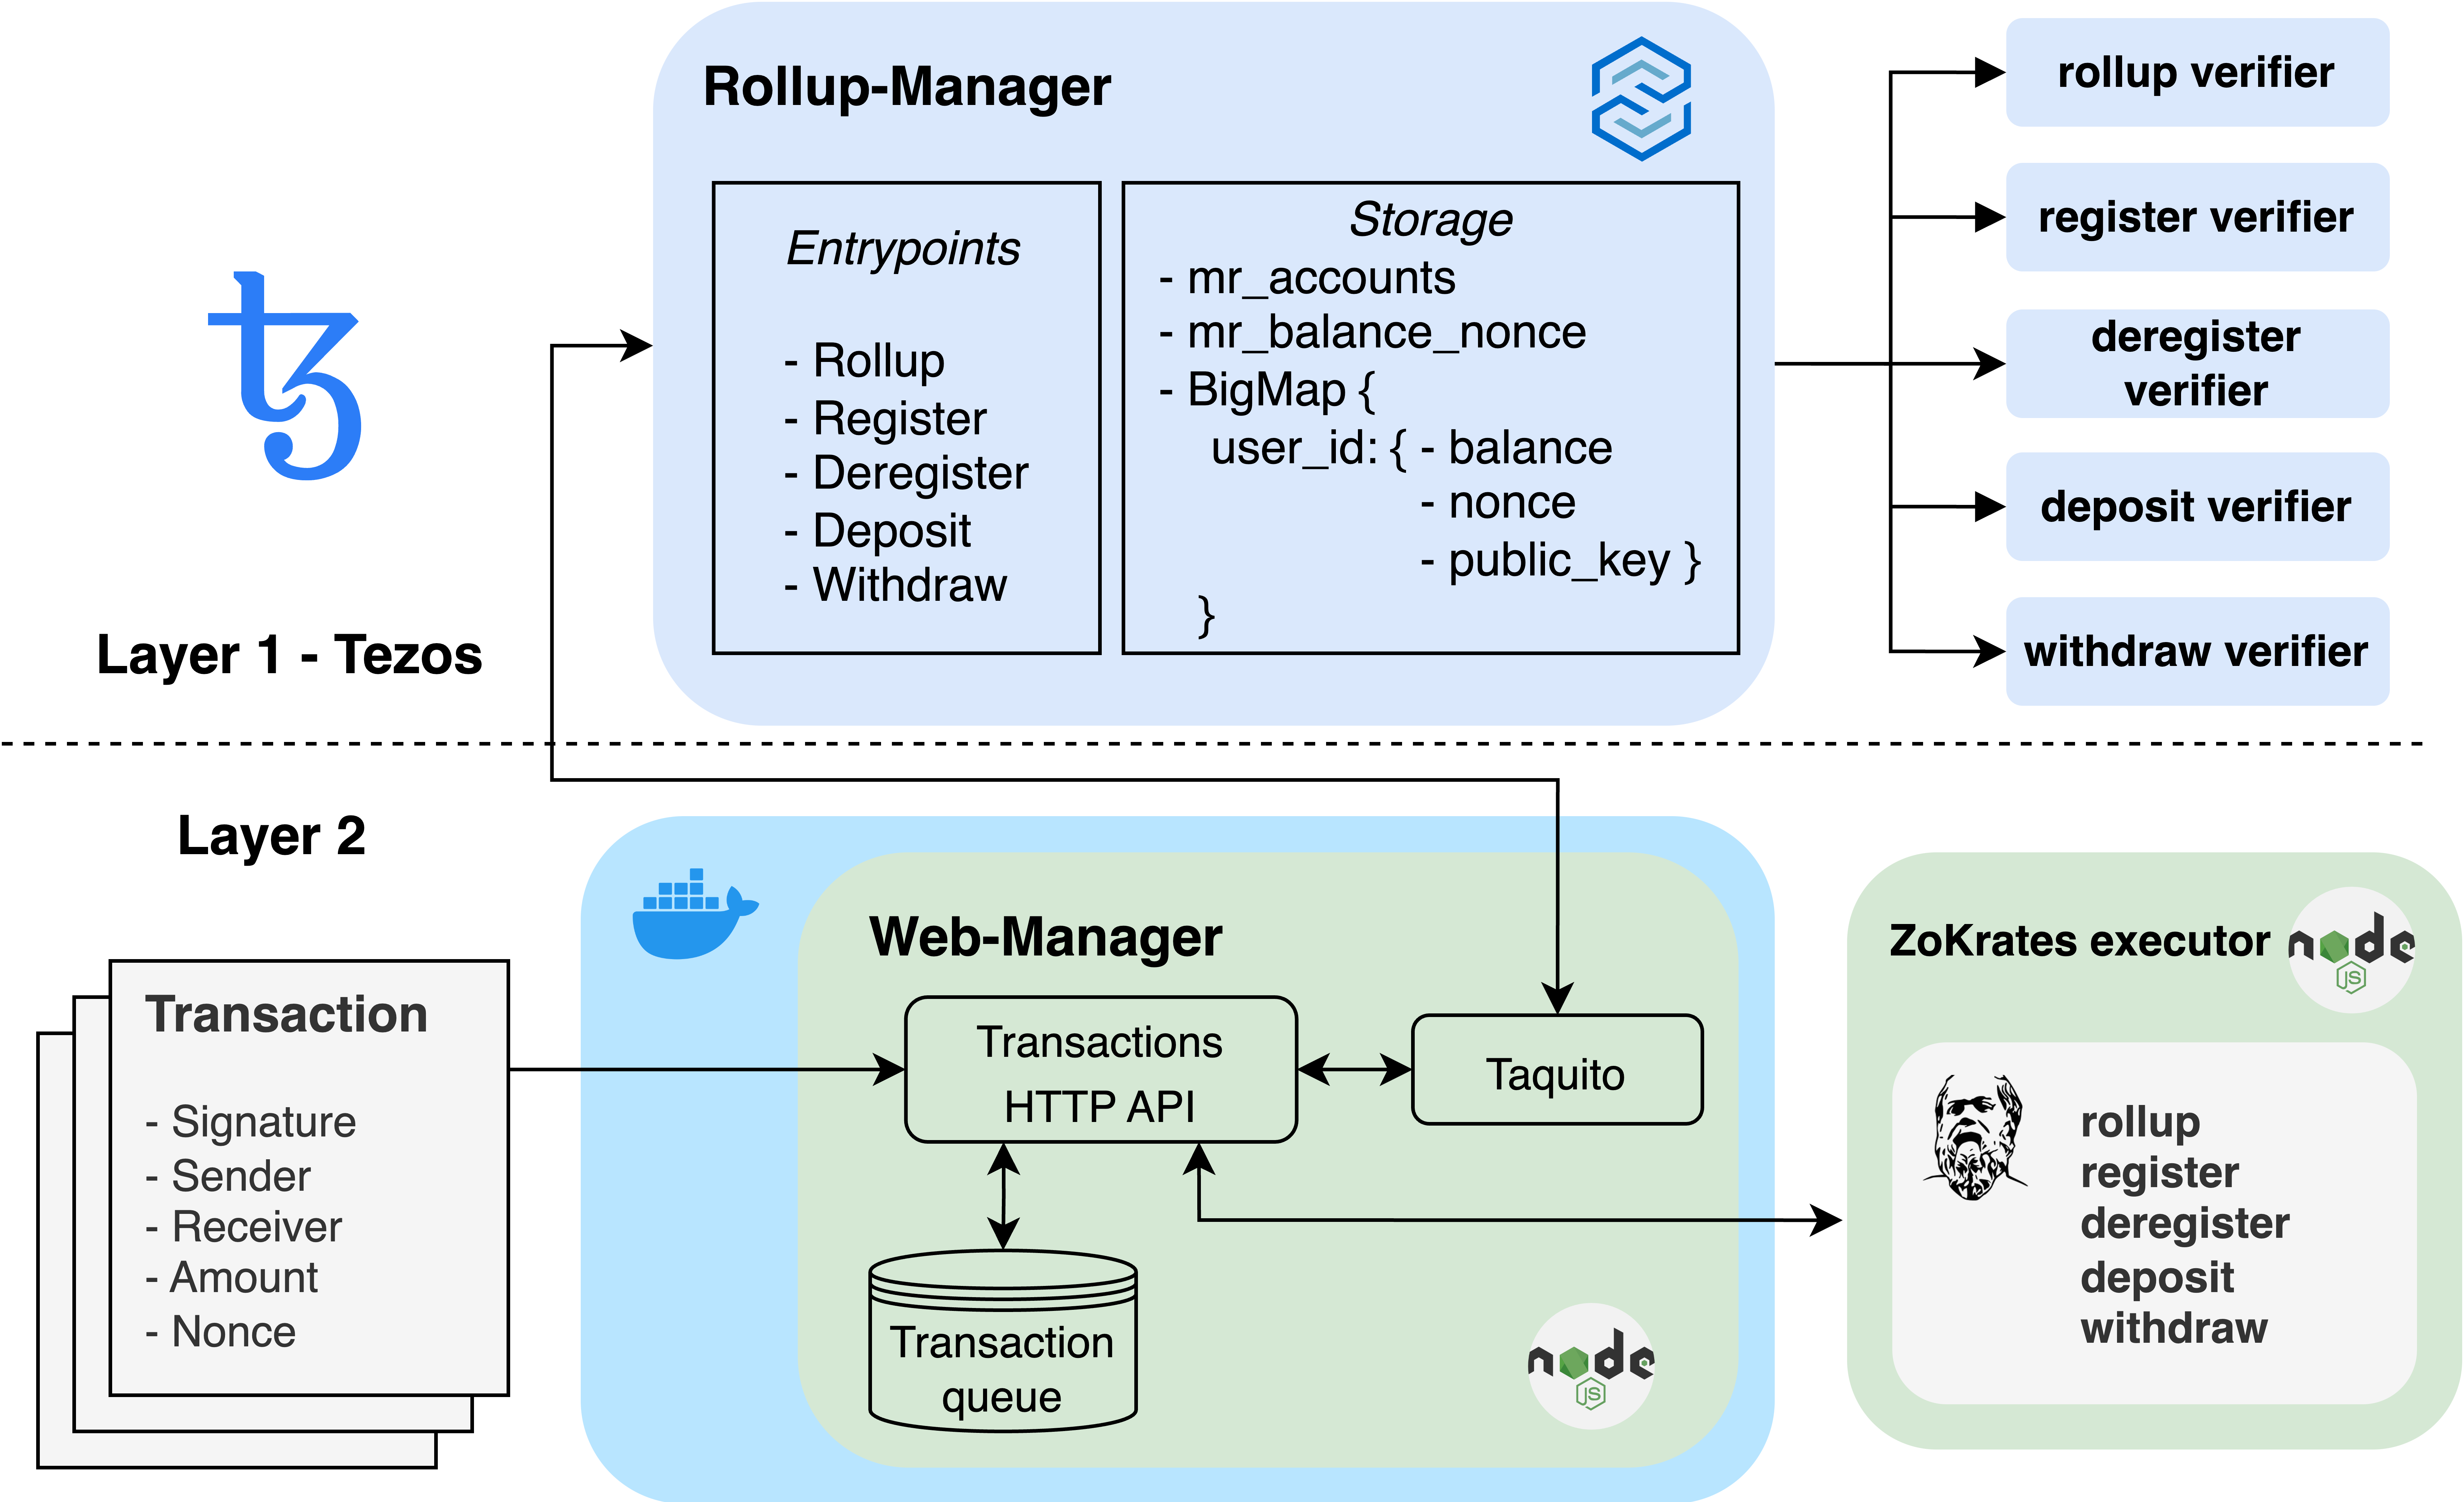
\includegraphics[width=0.9\columnwidth]{5_drawings-final_rollup_architecture.png}
	\caption[Scaling Solutions]{Architecture of the Rollup System.}  
	\label{fig:fig:5_drawings-final_rollup_archotecture.png}
  \end{figure} 

\section{Technologies\label{sec:technologies}}

The blockchain components are constructed utilizing the Tezos blockchain\footnote{\url{https://tezos.com/}} and the SmartPy\footnote{\url{https://smartpy.io/}} smart contract language. The Rollup System is deployed on the Tezos Ghostnet test network.

To engineer the Layer 2 components, web servers are developed using nodejs and Typescript running in Docker containers. The implementation of Rollup programs is accomplished through the utilization of the ZoKrates toolbox\footnote{\url{https://github.com/ZoKrates/ZoKrates}}, a comprehensive zk-SNARKs toolkit designed to facilitate the creation of verifiable computation programs.

The interaction between the Layer 2 and Layer 1 is made possible through the utilization of the Taquito\footnote{\url{https://tezostaquito.io/}} library, a TypeScript library that provides a simple interface for interacting with the Tezos blockchain.

Those technologies were already decided at the time of the project's inception, as they were the most suitable for the project's objectives. The Tezos blockchain was chosen due to its easy development and deployment, as well as the missing Layer 2 solutions.
\todo[inline]{Write why ZoKrates was chosen}

\section{Repeated Transactions Attack}
\label{sec:repeatedtransactionsattack}

To mitigate the risk of an attacker initiating repeated transactions, the nonce mechanism comes into play: each account holds a nonce, stored on Layer 1. When a transaction is submitted, it must include a nonce incremented by one, thereby facilitating the validation of transaction execution history.

Within the ZoKrates environment, proving the usage of updated balances and nonces necessitates computation of a merkle tree for the provided balance and nonce lists. This implies calculating two full binary trees, thereby increasing complexity. A workaround involves concatenating and hashing balances and nonces for individual users, forming a single merkle tree of these concatenated values. This approach incurs only the complexity of the concatenation function, involving a number of hashes equivalent to the number of accounts, ultimately substantiating the updated balances and nonces.

Changes were introduced to the rollup execution to incorporate the computation of new nonces alongside new balances. It's essential that ZoKrates receives transactions ordered by nonce for each user. While transactions from diverse users can be received, those from a single user must be ordered by nonce. The algorithm for verifying transaction nonces and calculating new nonces is as follows:
\begin{itemize}
	\item Initialize \textit{nonce\_array} and \textit{balance\_array}, with the current nonces and balances of all users;
	\item Iterate through the transactions:
	\begin{itemize}
		\item Check in \textit{nonce\_array} if the transaction nonce equals the sender's nonce plus one;
		\item If true:
		\begin{itemize}
			\item Increment senders's nonce in array \textit{nonce\_array};
			\item Decrement sender's balance in array \textit{balance\_array};
			\item Increment receiver's balance in array \textit{balance\_array};
			\item Proceed to next transaction;
		\end{itemize}
		\item If false:
		\begin{itemize}
			\item Fail program execution.
		\end{itemize}
    \end{itemize}
\end{itemize}

This approach accommodates multiple transactions from the same user, thwarting duplicate transaction execution.

The rollup execution complexity experiences minimal augmentation, as the nonce check coincides with balance calculation in the same loop, facilitating direct array access and preserving an O(n) complexity.

\section{Hash Function}

Hash functions play a crucial role in the Rollup execution process. They are extensively used for various tasks such as creating Merkle Trees, concatenating balances and nonces, and verifying signatures. One widely supported hashing function in this context is SHA-256. The initial implementation of the Rollup system employed the SHA-256 function provided by the ZoKrates toolbox. However, as demonstrated in Section \ref{subsec:6_hashfunc}, the use of this function introduces a significant number of constraints to the compiled Zokrates program, resulting in exponential complexity during execution. This inefficiency arises from the fact that classical cryptographic schemes predominantly consist of boolean operations, which become inefficient within a ZK-SNARK circuit \cite{belles-munoz_twisted_2021}.

A more recent hash function, known as Poseidon \cite{grassi_poseidon_nodate}, has been developed with a specific focus on efficiency within zk-SNARK circuits. By transitioning the Rollup system's hash function from SHA-256 to Poseidon, the number of constraints added to the program has been reduced by a factor of 100.

Notably, the adoption of the Poseidon hash function necessitates a revision of the system storage. While SHA-256 operates on 256-bit blocks, Poseidon operates on field sizes defined by the underlying elliptic curve. Additionally, considering the process of signature verification, the payload of a signed message must be hashed to fit a predetermined size prior to verification. In the case of Zokrates signature verification, which expects 512 bits of data, padding must be added after hashing the payload with Poseidon. This is due to the fact that the bls12\_381 curve on ZoKrates operates on a 254-bit field size. To meet the expected size, a padding of 258 bits, filled with zeros, is appended to the right of the payload's hash.

\section{Proof Reduction and Compression}
When creating ZoKrates' private and verification keys it is important to note that the size of the keys is proportional to the number of outputs that the ZoKrates program has. When executing a Rollup the outputs are the new Merkle Tree of the concatenated balances and nonces, plus the list of balances and nonces. Those values are in fact used to update the internal state on the Smart Contract living in Layer 1. As described in \ref{sec:3_smartContractsRequirements} the whole operation sent to the blockchain must not exceed 32768 bytes. Section \ref{subsec:6_verifierproofsize} shows how the proof size increases out of control when the number of users increases. This leads to the impossibility of sending the proof to the Rollup Smart Contract, making the system unusable. A proposed solution consists of realizing a reduction and compression of the outputs of the zokrates program.

\subsection{Proof Size Reduction}

To achieve a reduction in the number of outputs from the ZoKrates program, a change is made in the program's logic. Instead of returning the entire list of balances and nonces, the program only returns the altered balances and nonces. This adjustment introduces the requirement for an index that can be used to identify users in the list.

For every transaction, certain information needs to be returned: the sender's index, balance, and nonce, as well as the receiver's index and balance. In a hypothetical rollup system with 4096 users and 128 transactions per rollup, the outputs of the ZoKrates program shrink from 8193 to 641 (inclusive of the Merkle Root). This reduction significantly cuts down the proof size. Notably, in a Rollup system, many users remain inactive, participating infrequently in the rollup. This dynamic creates a considerable gap between the registered user count and the number of transactions, which enables this mechanism.

Furthermore, this approach proves more advantageous when a single user initiates multiple transactions to the same recipient, as the sender's index and balance are only returned once.

\subsection{Reducing Proof Size}

ZoKrates allows operating on fields of size 254 bits. The proof itself is made up of entries in these fields, no matter the original type of value. Even a simple boolean or a 254-bit value gets represented using just one field entry. This applies to lists of changed indexes, balances, and nonces too. When returning the list of modified indexes, balances and nonces they will occupy a single field value for just 32 bit of information.

By combining indexes, balances, and nonces into one field value, we can fit more info in a single entry. This merging cuts down the number of field entries from the ZoKrates program, which in turn shrinks the proof size. Here's a snippet of how this compression works within the ZoKrates program:

\begin{lstlisting}[language=C++]
field[NUM_TRANSACTIONS] mut result = [0; NUM_TRANSACTIONS];
for u32 i in 0..NUM_TRANSACTIONS {
  // Calculate new balances and nonce
  ......
  // Compress indexes, balances, and nonces
  bool[32] index_send_bits = u32_to_bits(index_sender);
  bool[32] balance_send_bits = u32_to_bits(balance_sender);
  bool[32] nonce_send_bits = u32_to_bits(nonce_sender);
  bool[32] index_rec_bits = u32_to_bits(index_receiver);
  bool[32] balance_rec_bits = u32_to_bits(balance_receiver);
  bool[254] joined = [
    ...index_send_bits, ...balance_send_bits,
    ...nonce_send_bits, ...[false; 94],
    ...index_rec_bits, ...balance_rec_bits
  ];
  result[i] = pack(joined);
}
\end{lstlisting}

This process returns one field value for each transaction. The first 96 bits hold sender-related data, followed by a 94-bit padding, and then 64 bits for receiver-related data.

Another way to improve this is by concatenating all data into one bit array, and then taking 254-bit chunks from it to create field values.

To get back the original values, the Smart Contract needs to decompress the data. At the moment, the ability to get data from field values as bytes is there, but the current SmartPy version lacks converting from Bytes to Nat. When that feature comes in, it wil be possible to restore original values from field values. The upcoming benchmarks will also account for the estimated cost of this value conversion.

\subsection{Storage}

Initially, the storage was designed with the intention of accommodating a limited number of users, employing a standard Map. It encompassed the following elements:
\begin{itemize}
	\item A Map of accounts indexed by a natural number, containing:
		\begin{itemize}
			\item A public key;
			\item A balance.
		\end{itemize}
	\item A list of 8 scalar values representing the Merkle Tree root of the accounts' public keys;
	\item A list of 8 scalar values representing the Merkle Tree root of the accounts' balances.
\end{itemize}

With scalability as a focal point, the storage structure was revamped to handle a growing user base through the adoption of a Big Map. This alteration is pivotal, given that the Big Map is lazily deserialized\footnote{\url{https://tezos.gitlab.io/michelson-reference/\#type-big_map}}, negating the need for gas during contract calls to deserialize the entire accounts Map. The storage now comprises:
\begin{itemize}
	\item A Big Map of accounts indexed by a natural number, encompassing:
		\begin{itemize}
			\item A public key;
			\item A balance;
			\item A nonce.
		\end{itemize}
	\item A list of 8 scalar values representing the Merkle Tree root of the accounts' public keys;
	\item A list of 8 scalar values representing the Merkle Tree root of the accounts' balances concatenated with their respective nonces.
\end{itemize}

Details on the nonce mechanism and the Merkle Tree roots are elucidated in Section \ref{sec:repeatedtransactionsattack}.

\subsection{ZoKrates Native Execution}
The execution of ZoKrates programs demands substantial resources, as evidenced in Section \ref{sec:benchmarks}. As a consequence, executing ZoKrates programs is allocated to a distinct server. This server operates as an independent entity, called upon by the primary Web Server. This strategy serves the dual purpose of optimizing resource allocation and facilitating scalability. Specifically, the architecture enables the isolation of resource-intensive tasks to a separate server, allowing efficient utilization and the ability to scale individual components as needed.

The primary server dispatches requests, inclusive of essential inputs sourced from the Manager smart contract, to the ZoKrates servers. These dedicated servers execute the ZoKrates programs, subsequently furnishing the results to the primary server. Notably, the utilization of a containerized environment for the ZoKrates server introduces challenges. The approach of running ZoKrates programs directly on the machine is chosen to mitigate the introduction of overhead stemming from OS-level virtualization, particularly relevant in scenarios involving pre-existing virtualized environments, such as cloud computing contexts. Figure \ref{fig:5_drawings-L2_technologies_ZoKrates_metal} illustrates the technologies of the new Layer 2 components.

\begin{figure}[ht]
	\centering
	\includegraphics[width=0.7\columnwidth]{5_drawings-L2_technologies_ZoKrates_metal.png}
	\caption[Scaling Solutions]{Technologies of the new Layer 2 components.}  
	\label{fig:5_drawings-L2_technologies_ZoKrates_metal}
  \end{figure} 


\section{New Features Implementation}
This section details the implementation of the new features of the project, including the problems encountered and the solutions devised.

\subsection{Registration and Deregistration}

This segment elucidates the registration and deregistration procedures for users. The primary objective is to add and remove users from storage, creating empty user entries during deregistration. This approach maintains user positioning within storage, allowing utilization of existing indexes.

Tezos supports optional types, enabling a value to be set as None, indicating its absence. This feature proves valuable during user removal from storage. The new storage Big Map, representing registered users, now comprises:
\begin{itemize}
	\item \textbf{index}: A natural number representing the user's index within storage;
	\item \textbf{mutez balance}: The user's balance;
	\item \textbf{nonce}: The user's nonce;
	\item \textit{optional} \textbf{public key}: The user's public key.
\end{itemize}

Given the resource-intensive nature of merkle tree generation, registration and deregistration processes are executed within dedicated ZoKrates programs and not in the smart contracts.

\subsubsection{Registration\label{subsec:registration}}

To register a new user, the two Merkle Trees must be recomputed, integrating the new user's public key, balance, and nonce. A ZoKrates program performs this computation, returning the new root hashes of both Merkle Trees. These hashes are then used by the manager smart contract to update the storage, incorporating new roots and the new user. The ZoKrates program requires the precise position for inserting the new user's data. This position is determined externally by a manager, which can communicate with an RPC to ascertain the first vacant slot within the storage's Big Map. The registration process verifies if the designated position holds an account with an empty key, balance, and nonce set to zero. Subsequently, the user's nonce is set to one, balance to zero, and public key to the user's public key.

\subsubsection{Deregistration}

Deregistration closely mirrors the registration process outlined in Section \ref{subsec:registration}. The ZoKrates deregistration program takes the user's index to be deregistered, along with other standard inputs. This program sets the user's public key to None, balance to zero, and nonce to zero. The updated root hashes of both Merkle Trees are returned by the deregistration program. The manager contract then employs these new roots to update storage, removing the user entry at the specified index.

\subsection{Deposit\label{subsec:deposit}}
The deposit process into the Layer 2 system is intricate due to the requirement of recalculating the merkle tree involving balances and nonces. As a result, the deposit procedure is divided into two distinct phases: the initial phase entails transferring funds from the user's account to the manager smart contract via a dedicated entrypoint call in the contract; the subsequent phase involves executing a ZoKrates program to recompute the merkle tree of balances and nonces, ultimately producing the new root of the tree. Figure \ref{fig:5_drawings-sequence_deposit.png} illustrates the deposit process.

\subsubsection{Phase 1: Transferring Funds to Manager Contract}
The deposit process is instigated by the user, who invokes the \textit{deposit} entrypoint within the manager contract and specifies the index of the account within the user Big Map. Subsequently, the manager contract facilitates the transfer of the designated sum from the user's account to its own account. Additionally, an internal record of pending deposits is maintained.

This internal deposit record adopts the structure of a \textit{Map (nat mutez)}, where the key corresponds to the user's index in the user Big Map, and the value signifies the sum of funds intended for deposition. This configuration accommodates the acceptance of multiple deposits from a single user, effectively tracking the specified deposit amounts.

In the aftermath of the first phase, the user remains unable to expend the transferred sum until the conclusion of the second phase.

\subsubsection{Phase 2: Merkle Tree Recalculation}
The second phase is initiated by a Web Server that detects a considerable accumulation of deposits in the deposit queue. Subsequently, the Web Server accesses the deposit list and initiates the ZoKrates program responsible for recalculating the merkle tree inclusive of the new deposits. Following this computation, the Web Server calls the \textit{receive\_deposit\_proof} entrypoint within the manager contract, providing the freshly computed merkle tree root as a parameter. Consequently, the manager contract updates the root of the merkle tree associated with balances and nonces, adjusts user balances to incorporate the deposited funds, and ultimately eradicates the deposits from the internal pending deposit list.

\begin{figure}[ht]
	\centering
	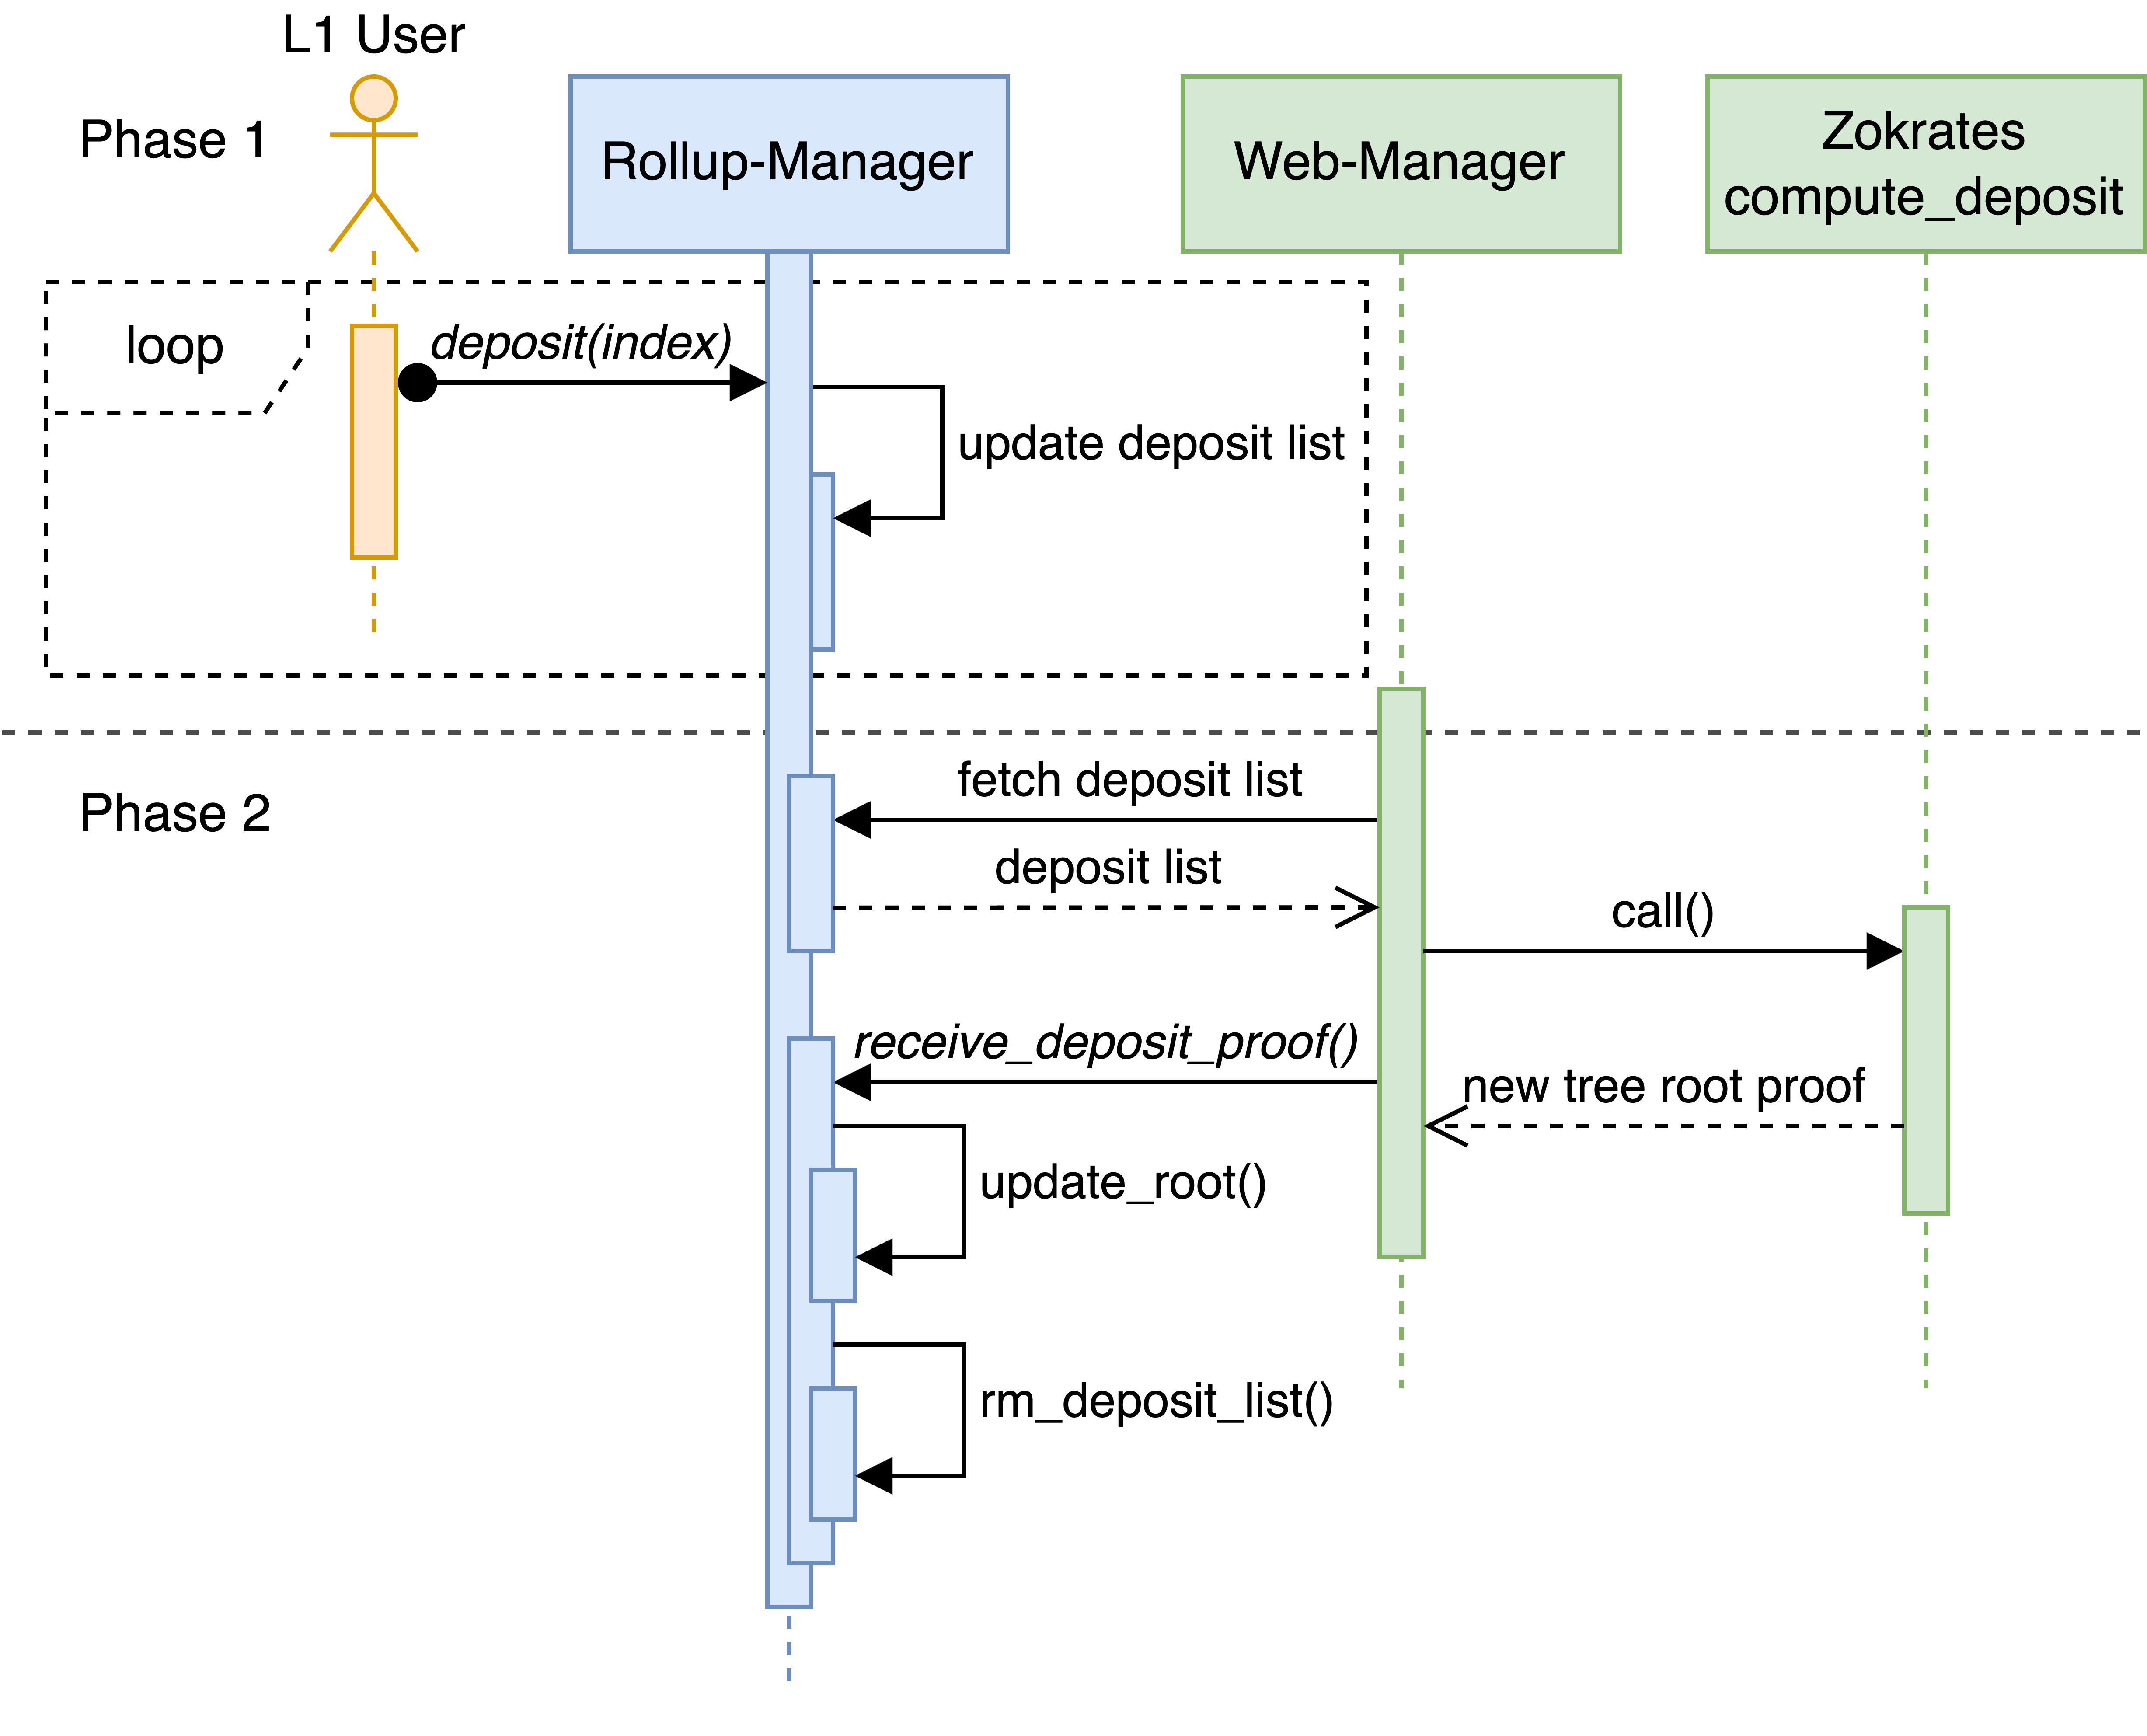
\includegraphics[width=0.7\columnwidth]{5_drawings-sequence_deposit.png}
	\caption[Scaling Solutions]{Sequence Diagram of Deposit Process}  
	\label{fig:5_drawings-sequence_deposit.png}
  \end{figure} 

  \subsection{Withdraw}
  This section delineates the Withdrawal process, enabling the movement of funds from the Layer 2 system to the Layer 1 system. The withdrawal process diverges from the deposit process expounded in Section \ref{subsec:deposit}. Notably, withdrawals operate within a single phase, a strategic choice that expedites the withdrawal procedure, affording users the prompt retrieval of their funds without the necessity of reaching a threshold of users in the withdrawal queue.
  
  The withdrawal initiation commences as users dispatch withdrawal requests to the Web Server. Subsequently, the Web Server retrieves the user's balance and nonce from the manager contract and generates withdrawal inputs for the dedicated ZoKrates program. This ZoKrates program orchestrates the computation of the new root hash for the merkle tree containing balances and nonces. This computation involves the subtraction of the user-specified amount. The computed new root hash is then relayed back to the Web Server. In turn, the Web Server invokes the \textit{receive\_withdrawal\_proof} entrypoint within the manager smart contract. This invocation encompasses the provision of the new root hash as a parameter.
  
  Within the manager contract, the merkle tree root hash undergoes an update, alongside adjustments to the user's balance and nonce. Subsequently, the requested sum is transferred to the user's account, finalizing the withdrawal process.
  


\section{Optimization}
During a preliminary testing phase of the Layer 2 system immediately emerged a problem when increasing the number of user from 4 to 8. The problem was the compute resources needed to compile and run the ZoKrates programs: with only 8 users the compilation of the programs required more than 100GB of RAM. Due to the structure of the merkle trees generation, only powers of 2 can be taken as number of users. The 

\begin{figure}[htb]
  \centering
  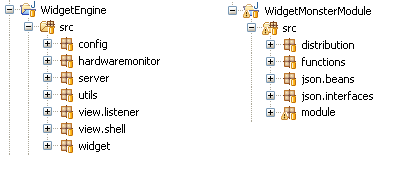
\includegraphics[width=10cm]{screenshot_2_projects}
  \caption{Project Structure}
  \label{fig:projects}
\end{figure}

\noindent
The following listing briefly describes the single packages of both projects in alphabetical order to give an overview of the implementation:
\\
\\
\textbf{config} 
\\
Lorem Ipsum...
\\
\\
\textbf{server} 
\\
Lorem Ipsum...
\\
\\
\textbf{utils} 
\\
Lorem Ipsum...

\section{Important Implementation Aspects\label{sec:implaspects}}

Do not explain every class in detail. Give a short introduction about the modules or the eclipse projects. If you want to explain relevant code snippets use the 'lstlisting' tag of LaTeX. Put only short snippets into your thesis. Long listing should be part of the annex.

\lstset{caption=JSON String Code Snippet,label=jsonstring,showstringspaces=false}
\begin{lstlisting}
{
	id: 1,
	method: "myInstance.getGroup",
	params: ["Teammates", 2, true]
}

{
	id: 2,
	result: [
		  "groupDesc":"These are my teammates",
		  {
			"javaClass":"src.package.MemberClass",
			"memberName": "Bob",      
		  }
		]
}\end{lstlisting}

You can also compare different approaches. Example: Since the implementation based on X failed I choosed to implement the same aspect based on Y. The new approach resulted in a much faster ...

\section{Graphical User Interface\label{sec:gui}}

Lorem Ipsum...

\section{Documentation\label{sec:docu}}

Lorem Ipsum...



    \chapter{Evaluation\label{cha:chapter6}}

In this chapter the implementation of Component X is evaluated. An example instance was created for every service. The following chapter validates the component implemented in the previous chapter against the requirements.
\\
\\
Put some screenshots in this section! Map the requirements with your proposed solution. Compare it with related work. Why is your solution better than a concurrent approach from another organization?

\section{Test Environment\label{sec:testenvir}}

Fraunhofer Institute FOKUS' Open IMS Playground was used as a test environment for the telecommunication services. The IMS Playground ...

\section{Scalability\label{sec:scal}}

Lorem Ipsum

\section{Usability\label{sec:usab}}

Lorem Ipsum

\section{Benchmarks\label{sec:benchmarks}}

Lorem Ipsum
    \chapter{Conclusion\label{cha:chapter7}}
% The final chapter summarizes the thesis. The first subsection outlines the main ideas behind Component X and recapitulates the work steps. Issues that remained unsolved are then described. Finally the potential of the proposed solution and future work is surveyed in an outlook.

% \section{Summary\label{sec:summary}}

% Explain what you did during the last 6 month on 1 or 2 pages!
% \\
% \\
% \noindent The work done can be summarized into the following work steps

% \begin{itemize}
% 		\item Analysis of available technologies
% 		\vspace{-0.11in} 
% 		\item Selection of 3 relevant services for implementation
% 		\vspace{-0.11in} 
% 		\item Design and implementation of X on Windows
% 		\vspace{-0.11in} 
% 		\item Design and implementation of X on mobile devices
% 		\vspace{-0.11in} 
% 		\item Documentation based on X
% 		\vspace{-0.11in} 
% 		\item Evaluation of the proposed solution
% \end{itemize}

% \section{Dissemination\label{sec:dissemination}}

% Who uses your component or who will use it? Industry projects, EU projects, open source...? Is it integrated into a larger environment? Did you publish any papers?

% \section{Problems Encountered\label{sec:problems}}

% Summarize the main problems. How did you solve them? Why didn't you solve them?

% \section{Outlook\label{sec:outlook}}

% Future work will enhance Component X with new services and features that can be used ...

% ---------------------------------------------------------------
\backmatter % no page numbering from here
    \todo[inline]{talk to your supervisor if this is needed}
    \addchap{List of Acronyms}

\begin{tabbing}
spacespacespace \= space \kill
3GPP	 \> 	3rd Generation Partnership Project	 \\
AJAX	\>	Asynchronous JavaScript and XML \\
API	 \> 	Application Programming Interface	 \\
AS	\>	Application Server \\
CSCF	 \> 	Call Session Control Function	 \\
CSS	\>	Cascading Stylesheets \\
DHTML	\>	Dynamic HTML \\
DOM	\>	Document Object Model \\
FOKUS	\>	Fraunhofer Institut fuer offene Kommunikationssysteme \\
GUI	\>	Graphical User Interface \\
GPS	\>	Global Positioning System \\
GSM	\>	Global System for Mobile Communication\\
HTML	\>	Hypertext Markup Language \\
HSS	 \> 	Home Subscriber Server	 \\
HTTP	 \> 	Hypertext Transfer Protocol	 \\
I-CSCF	 \> 	Interrogating-Call Session Control Function	 \\
IETF	\>	Internet Engineering Task Force \\
IM	\>	Instant Messaging \\
IMS	 \> 	IP Multimedia Subsystem	 \\
IP	 \> 	Internet Protocol	 \\
J2ME	\>	Java Micro Edition \\
JDK	\>	Java Developer Kit \\
JRE	\>	Java Runtime Environment \\
JSON	\>	JavaScript Object Notation \\
JSR	\>	Java Specification Request \\
JVM	 \> 	Java Virtual Machine	 \\
NGN	 \> 	Next Generation Network	 \\
OMA	 \> 	Open Mobile Alliance	 \\
P-CSCF	 \> 	Proxy-Call Session Control Function	 \\
PDA	\>	Personal Digital Assistant \\
PEEM	 \> 	Policy Evaluation, Enforcement and Management	 \\
QoS	 \> 	Quality of Service	 \\
S-CSCF	 \> 	Serving-Call Session Control Function	 \\
SDK	\>	Software Developer Kit \\
SDP	\>	Session Description Protocol \\
SIP	 \> 	Session Initiation Protocol	 \\
SMS	\>	Short Message Service \\
SMSC	\> Short Message Service Center \\
SOAP	 \> 	Simple Object Access Protocol	 \\
SWF	\>	Shockwave Flash \\
SWT	\>	Standard Widget Toolkit \\
TCP	 \> 	Transmission Control Protocol	 \\
Telco API	\>	Telecommunication API \\
TLS	\>	Transport Layer Security \\
UMTS	 \> 	Universal Mobile Telecommunication System	 \\
URI	 \> 	Uniform Resource Identifier	 \\
VoIP	 \> 	Voice over Internet Protocol	 \\
W3C	 \> 	World Wide Web Consortium	 \\
WSDL	\>	Web Service Description Language \\
XCAP	 \> 	XML Configuration Access Protocol	 \\
XDMS	 \> 	XML Document Management Server	 \\
XML	 \> 	Extensible Markup Language	 \\
\end{tabbing}
\endinput

		
		% if you want to provide a glossary with explanations of important terms put it in here

    \bibliographystyle{geralpha}
    \bibliography{./bib/manual}
    
    \addchap{Annex}

\begin{appendix}

\lstset{language=,caption=Sourcecode Listing,captionpos=b,
label=yahoowidgetkon,showstringspaces=false,
basicstyle={\fontfamily{pcr}\selectfont\footnotesize}}
\begin{lstlisting}
<?xml version="1.0" encoding="UTF-8"?>
<widget>
	 <debug>off</debug>
	 <window name="myWindow" title="Hello Widget" visible="true">
		 <height>120</height>
		 <width>320</width>
		 <image src="Resources/orangebg.png">
			<name>orangebg</name>
			<hOffset>0</hOffset>
			<vOffset>0</vOffset>
		</image>
		 <text>
			 <name>myText</name>
			 <data>Hello Widget</data>
			 <color>#000000</color>
			 <size>20</size>
			 <vOffset>50</vOffset>
			 <hOffset>120</hOffset>
		 </text>
	</window>
</widget>
\end{lstlisting}

\newpage


\lstset{caption=SIP request and response packet\cite{SIPBook},
captionpos=b,label=sippacket,showstringspaces=false,
basicstyle={\fontfamily{pcr}\selectfont\footnotesize}}
\begin{lstlisting}
INVITE sip:bob@network.org SIP/2.0
Via: SIP/2.0/UDP 100.101.102.103:5060;branch=z9hG4bKmp17a
Max-Forwards: 70
To: Bob <sip:bob@network.org>
From: Alice <sip:alice@ims-network.org>;tag=42
Call-ID: 10@100.101.102.103
CSeq: 1 INVITE
Subject: How are you?
Contact: <sip:xyz@network.org>
Content-Type: application/sdp
Content-Length: 159
v=0
o=alice 2890844526 2890844526 IN IP4 100.101.102.103
s=Phone Call
t=0 0
c=IN IP4 100.101.102.103
m=audio 49170 RTP/AVP 0
a=rtpmap:0 PCMU/8000

SIP/2.0 200 OK
Via: SIP/2.0/UDP proxy.network.org:5060;branch=z9hG4bK83842.1
;received=100.101.102.105
Via: SIP/2.0/UDP 100.101.102.103:5060;branch=z9hG4bKmp17a
To: Bob <sip:bob@network.org>;tag=314159
From: Alice <sip:alice@network.org>;tag=42
Call-ID: 10@100.101.102.103
CSeq: 1 INVITE
Contact: <sip:foo@network.org>
Content-Type: application/sdp
Content-Length: 159
v=0
o=bob 2890844526 2890844526 IN IP4 200.201.202.203
s=Phone Call
c=IN IP4 200.201.202.203
t=0 0
m=audio 49172 RTP/AVP 0
a=rtpmap:0 PCMU/8000
\end{lstlisting}


\end{appendix}

\endinput


\end{document}
